\documentclass[preprint,
3p]{elsarticle} %review=doublespace preprint=single 5p=2 column
%%% Begin My package additions %%%%%%%%%%%%%%%%%%%

\usepackage[hyphens]{url}

  \journal{Computers \& Education} % Sets Journal name

\usepackage{graphicx}
%%%%%%%%%%%%%%%% end my additions to header

\usepackage[T1]{fontenc}
\usepackage{lmodern}
\usepackage{amssymb,amsmath}
% TODO: Currently lineno needs to be loaded after amsmath because of conflict
% https://github.com/latex-lineno/lineno/issues/5
\usepackage{lineno} % add
\usepackage{ifxetex,ifluatex}
\usepackage{fixltx2e} % provides \textsubscript
% use upquote if available, for straight quotes in verbatim environments
\IfFileExists{upquote.sty}{\usepackage{upquote}}{}
\ifnum 0\ifxetex 1\fi\ifluatex 1\fi=0 % if pdftex
  \usepackage[utf8]{inputenc}
\else % if luatex or xelatex
  \usepackage{fontspec}
  \ifxetex
    \usepackage{xltxtra,xunicode}
  \fi
  \defaultfontfeatures{Mapping=tex-text,Scale=MatchLowercase}
  \newcommand{\euro}{€}
\fi
% use microtype if available
\IfFileExists{microtype.sty}{\usepackage{microtype}}{}
\usepackage[]{natbib}
\bibliographystyle{elsarticle-num}

\ifxetex
  \usepackage[setpagesize=false, % page size defined by xetex
              unicode=false, % unicode breaks when used with xetex
              xetex]{hyperref}
\else
  \usepackage[unicode=true]{hyperref}
\fi
\hypersetup{breaklinks=true,
            bookmarks=true,
            pdfauthor={},
            pdftitle={From heartbeat to data -- Using wearable fitness trackers as an affordable approach to assess teacher stress},
            colorlinks=false,
            urlcolor=blue,
            linkcolor=magenta,
            pdfborder={0 0 0}}

\setcounter{secnumdepth}{5}
% Pandoc toggle for numbering sections (defaults to be off)


% tightlist command for lists without linebreak
\providecommand{\tightlist}{%
  \setlength{\itemsep}{0pt}\setlength{\parskip}{0pt}}




\usepackage{hyperref}
\hypersetup{colorlinks=true, linkcolor=blue, citecolor=blue, urlcolor=blue}
\setcitestyle{numbers}
\usepackage{tabularx}
\usepackage{threeparttable}
\usepackage{booktabs}
\usepackage{array}
\usepackage{caption}
\usepackage{tablefootnote}
\usepackage{float}
\usepackage{wrapfig}
\usepackage{pdflscape}
\usepackage{longtable}
\usepackage{geometry}
\usepackage{caption}



\begin{document}


\begin{frontmatter}

  \title{From heartbeat to data -- Using wearable fitness trackers as an
affordable approach to assess teacher stress}
    \author[Leipzig University]{Mandy Klatt%
  \corref{cor1}%
  \fnref{1}}
   \ead{mandy.klatt@uni-leipzig.de} 
    \author[Leipzig University]{Christin Lotz%
  %
  \fnref{2}}
   \ead{christin.lotz@uni-leipzig.de} 
    \author[UoG, DZKJ]{Peer Keßler%
  %
  \fnref{3}}
   \ead{peer.kessler@uni-greifswald.de} 
    \author[Leipzig University]{Gregor Kachel%
  %
  \fnref{4}}
   \ead{gregor.kachel@gmail.com} 
    \author[Leipzig University]{Anne Deiglmayr%
  %
  \fnref{5}}
   \ead{anne.deiglmayr@uni-leipzig.de} 
      \affiliation[Leipzig University]{
    organization={Leipzig University Division of Empirical School and
Classroom Research, Institute of Educational
Sciences},addressline={Marschnerstr.
29},city={Leipzig},postcode={04109},country={Germany},}
    \affiliation[UoG]{
    organization={University of Greifswald, Division of Health and
Prevention, Institute of Psychology},addressline={Robert-Blum-Str.
13},city={Greifswald},postcode={17489},country={Germany},}
    \affiliation[DZKJ]{
    organization={German Center for Child and Adolescent Health
(DZKJ)},addressline={Robert-Blum-Str.
13},city={Greifswald},postcode={17489},country={Germany},}
    \cortext[cor1]{Corresponding author}
    \fntext[1]{Conceptualization, Methodology, Formal analysis,
Investigation, Data Curation, Writing - Original Draft}
    \fntext[2]{Conceptualization, Methodology, Writing - Review \&
Editing, Supervision}
    \fntext[3]{Conceptualization, Methodology, Writing - Review \&
Editing}
    \fntext[4]{Formal analysis, Data Curation, Writing - Review \&
Editing}
    \fntext[5]{Conzeptualization, Methodology, Writing - Review \&
Editing, Supervision}
  
  \begin{abstract}
  Past research on physiological indicators of teacher stress often had
  to rely on expensive and obtrusive assessment methods. Modern fitness
  trackers represent a non-invasive and convenient alternative. This
  study investigated the use of wrist-worn fitness trackers to assess
  teacher heart rate (HR) as an indicator of stress during teaching. In
  a laboratory study, we used a Fitbit® fitness tracker to assess
  teachers´ HR before, during, and after a potentially stressful
  micro-teaching session. Our results demonstrate that the fitness
  tracker was indeed useful for mapping teachers' stress, with the data
  showing how teachers' HR increased before, peaked during, and
  progressively decreased after the micro-teaching session. Moreover, we
  related the fitness tracker data to retrospective teacher
  self-reports. We found that teachers' subjective stress appraisals,
  together with their teaching experience, explained only small amounts
  of variance in HR data. We discuss the potential of fitness trackers
  as an affordable and ubiquitous assessment tool for research on
  teacher stress in the classroom and provide advice for practical
  implementation.
  \end{abstract}
    \begin{keyword}
    teacher stress \sep fitness tracker \sep heart rate \sep classroom
disruptions \sep wearable technology \sep 
    physiological stress measurement
  \end{keyword}
  
 \end{frontmatter}

\section{Introduction}\label{introduction}

The teaching profession is one of the most stressful professions, with
teachers facing a host of stressors during their everyday work
\citep{smith2000, herman2020, schult2014belastet}. To better understand
mechanisms in teacher stress, there is a growing research interest in
physiological measures such as heart rate (HR) as online measures of
teachers' stress during teaching
\citep{karner2021teachers, wettstein2020ambulatory}. For example, it has
been shown that teacher-centered activities and typical
classroom-related stressors increase teacher HR during teaching
activities
\citep{sperka1995, scheuch1997psychophysische, donker2018, junker2021, huang2022class}.
However, previous studies have often relied on expensive and obtrusive
electrocardiographs (ECG). Modern fitness trackers represent a
non-invasive and convenient alternative \citep{ferguson2015}.

Classroom disruptions are a major stressor in teachers' daily work
\citep{boyle1995structural, aloe2014multivariate}, and learning how to
deal with them is an important aspect of professional expertise
\citep{wolff2015keeping}. According to \citet{lazarus1990theory}
transactional model of stress and coping, the experience of stress in
response to stressors such as classroom disruptions depends on the
teacher's subjective appraisal, which, in turn, depends on their coping
resources, such as their professional knowledge. The resulting stress
response has a psychological, physiological, or behavioral dimension
\citep{kyriacou1978}. Therefore, in order to better understand how
classroom stressors affect teachers' stress response, subjective
self-reports should be accompanied by objective, physiological measures
\citep{wettstein2021}. Teachers' use of wrist-worn fitness trackers in
educational research provides fine-grained, in vivo data, allowing
researchers as well as teachers themselves to monitor their
physiological stress response continuously during teaching, across
settings, and at low costs. Being able to monitor, and eventually
counteract, teacher stress levels appears particularly relevant given
the profession's generally high stress levels and associated negative
health effects \citep{johnson2005experience, montgomery2005meta}. To
harness this potential, the present study explored the use of
wrist-based fitness trackers as a tool to assess teachers' HR, as an
indicator of stress, before, during, and after a teaching session during
which typical, potentially stressful, classroom disruptions occurred.
Further, we explored to what extent teachers' subjective appraisals of
classroom disruptions and their teaching experience predicted teacher
stress as assessed by the fitness tracker.

\subsection{Fitness trackers as a ubiquitous, low-cost tool for
assessing physiological stress
responses}\label{fitness-trackers-as-a-ubiquitous-low-cost-tool-for-assessing-physiological-stress-responses}

Fitness trackers provide data on physical activity and cardiovascular
parameters such as HR, supporting personalized fitness goals
\citep{nuss2021effects} and stress management \citep{hao2018chrv}. They
can be used as ubiquitous, low-cost, and unintrusive data collection
instruments \citep{godfrey2018z}, and their wide-spread use and everyday
availability align with the increasing popularity and acceptance of
wearables among the general population \citep{peng2022acceptance}. In
contrast to self-reported questionnaires on stress
\citep{chaplain2008, liu2020} that are prone to biases like social
desirability \citep{razavi2001self} or recall errors
\citep{van2016accuracy}, fitness trackers, as ambulatory assessment
methods \citep{trull2013ambulatory, wettstein2020ambulatory}, offer more
objective insights into teachers' stress levels by monitoring teachers'
physiological stress responses without disrupting teaching
\citep{donker2018, runge2020}.

One important health parameter assessed by nearly all wrist-worn fitness
trackers is heart rate \citep{scalise2018wearables}. HR indicates the
number of heartbeats within one minute and is typically expressed as
beats per minute (BPM)
\citep{berntson2007cardiovascular, hottenrott2007}. At rest, the average
HR of adults typically ranges between 60 and 80 BPM
\citep{sammito2015guideline}. HR can be detected and measured in
different ways using sensors, such as electrocardiography (ECG) or
photoplethysmography (PPG) \citep{mukhopadhyay2017wearable}. While ECG
sensors offer precise measurements by detecting the heart's electrical
activity, their intrusive nature and requirement of direct skin contact
may limit their suitability \citep{kranjec2014non}, particularly in
educational settings. In contrast, photoplethysmography (PPG) is a
rather uncomplicated and inexpensive technique to measure HR, commonly
found in commercially available fitness trackers
\citep{castaneda2018review}. This optical method assesses HR by flashing
green or red lights to measure changes in blood volume in the
capillaries of the skin \citep{allen2007photoplethysmography}.

Physiologically, HR is regulated by the sympathetic and parasympathetic
nervous systems \citep{pham2021}. An increase in sympathetic activity
results in HR being sped up (``fight or flight'' response)
\citep{taelman2009influence}; whereas an increase in parasympathetic
activity results in HR being slowed down (``rest and digest'' response,
\citet{battipaglia2015}). Stress or mental and physical strain directly
increases HR \citep{custodis2014heart, sachs2014}. Therefore, an
increase in HR can be regarded as an indicator of increasing stress, and
a decrease as an indicator of relaxation and ease \citep{kyriacou1978}.
Thus, fitness trackers offer low-cost and unobtrusive access to
psychological stress data.

\subsection{HR in teaching-learning
contexts}\label{hr-in-teaching-learning-contexts}

Prior research, typically using ECG methods, has shown that changes in
teachers' HR can be mapped onto stressors they experience during
teaching. For example, teachers' HR tends to increase when teachers take
an exposed position in student-teacher interaction
\citep{sperka1995, scheuch1997psychophysische, donker2018, junker2021}.
\citet{sperka1995} for example recorded the HR of 16 pre-service
teachers during their first lesson and showed that teachers' HR
increased significantly during teaching. The activation was particularly
prominent at the beginning of the lesson and decreased over the course
of the lesson. The authors suggested that pre-service teachers'
proactive coping strategies, such as actively managing student
interactions, helped lower their HR levels. Other ECG studies identified
typical stressors predicting increases in HR, such as class size
\citep{huang2022class}, or low student engagement and motivation
\citep{junker2021}. \citet{junker2021} recorded the HR of 40 teachers
during a real classroom lesson. Again, teacher stress, induced by
factors such as low student engagement (e.g., lack of motivation or
interest in tasks) or teacher-centered activities (e.g., teacher-focused
classroom activities), resulted in elevated HR.

More recent studies have begun using wrist-worn fitness trackers to
investigate HR trends in instructional settings
\citep{Darnell2019, chalmers2021}. \citet{Darnell2019} measured the HR
of 15 medical college students listening to lectures, using wrist-worn
devices. The analysis revealed a constant decrease in HR throughout the
lecture, with HR peaks during more interactive learning phases.
\citet{chalmers2021} used HR data from a fitness tracker to identify
physiological changes during stress-inducing tasks (i.e., the Trier
Social Stress Test; \citet{kirschbaum1993trier}). Average HR increased
significantly from the resting to the stress inducing phases. Even
though the participants of these previous studies
\citep{Darnell2019, chalmers2021} were not teachers but learners, the
results are relevant for studying teacher stress as they demonstrated
that HR can be effectively recorded using fitness trackers over the
course of a whole learning unit, and HR changes are in line with the
occurrence of activating or stress-inducing tasks.

To the best of our knowledge, only one study has directly assessed
teachers' HR during teaching using a wrist-worn fitness tracker:
\citet{runge2020} assessed HR as an indicator of stress in four
in-service teachers during authentic lessons. They used fitness
trackers' recordings to create a profile for each teacher, with the aim
of differentiating between teachers reporting higher vs.~lower levels of
stress. It was found that the combination of a high HR, a high number of
steps, and short sleep duration was characteristic for teachers
reporting high stress levels. However, it should be noted that the
generalizability of these results is limited due to the small sample
size.

In summary, previous studies have revealed that teachers' (and
students') HR changes depend on their activities and the stressors they
experience, with an increase in HR already before the expected stressors
occur, and with peaks in activating phases
\citep{Darnell2019, chalmers2021}. For teachers, teacher-centered phases
led to an increase in HR
\citep{sperka1995, scheuch1997psychophysische, donker2018, junker2021}.
However, there is a lack of studies using teacher-worn fitness trackers
in larger samples, exploring the feasibility of this convenient tool for
researching links between teachers' HR and stress inducing events and
mechanisms.

\subsection{A model of teacher stress}\label{a-model-of-teacher-stress}

According to \citet{kyriacou1978}, teacher stress can be defined as a
negative affective response, typically accompanied by physiological
changes such as increased HR, triggered by job-related demands, and
perceived as threatening to one's self-esteem or well-being. Coping
mechanisms help to reduce the perceived threat. Kyriacou's definition of
teacher stress (see \citet{kyriacou1978} and, for a more recent
adaptation, \citet{van2006stress}) is based on the transactional stress
model by Lazarus and colleagues
\citep{lazarus1966psychological, lazarus1990theory}, which highlights
the interaction between an individual and the environment, whereby
stress refers to a person's subjective reaction to an event (a stressor)
that exceeds the person's adaptive resources.

Fig.\ref{fig.1} shows, in a simplified way, how classroom events affect
teachers' stress level, according to the adaptation of the Lazarus model
to teacher stress proposed by \citet{van2006stress}: When potential
stressors (e.g., classroom disruptions) occur during teaching (1),
teachers intuitively judge how disruptive the event is in a primary
appraisal (2). If potential stressors are judged as threatening, i.e.,
as actual stressors (3), teachers consider whether they have sufficient
resources for coping with the stressors (4). Teachers utilize these
resources in trying to cope with the stressors, e.g., by employing
classroom management strategies (5). In cases when coping fails, stress
ensues, often accompanied by physiological reactions like increased HR
(6). As part of the coping process, and dependent on its outcomes,
teachers re-evaluate the stressor (7).

As shown in Fig.\ref{fig.1}, teachers' primary and secondary appraisal
as well as coping attempts are influenced by professional experience. As
professional experience grows, teachers develop cognitive scripts for
managing classroom events, resulting in more complex and problem-focused
classroom management skills \citep{wolff2021classroom}, and thus more
effective coping and less stress. Empirically, classroom management
skills and problem-focused coping styles are linked to fewer instances
of emotional exhaustion \citep{maslach2001job, clunies2008self}. Novices
in the teaching profession, on the other hand, face considerable stress
and often feel overwhelmed by the demands of teaching
\citep{ophardt2017klassenmanagement, wolff2015keeping, klusmann2012berufliche}
with many leaving the profession within the first five years
\citep{ingersoll2003}. Accordingly, when resources are lacking and
coping fails, negative consequences for health (e.g., burnout) and for
work (e.g., high turnover rates) can arise
\citep{jalongo2006, unterbrink2007, aloe2014multivariate}, highlighting
the importance of professional expertise for managing teacher stress
\citep{fisher2011}.

\captionsetup[figure]{
    labelsep=colon,      % Period after Figure label
    font=footnotesize,           % Smaller font size for APA style
    justification=justified, % Left-justified captions, as per APA guidelines
    singlelinecheck=false % Avoid centering if the caption is single-line
}

\captionsetup[table]{
    labelsep=colon,      % Period after Figure label
    font=footnotesize,           % Smaller font size for APA style
    justification=justified, % Left-justified captions, as per APA guidelines
    singlelinecheck=false % Avoid centering if the caption is single-line
}

\begin{figure}[htbp]
  \centering
  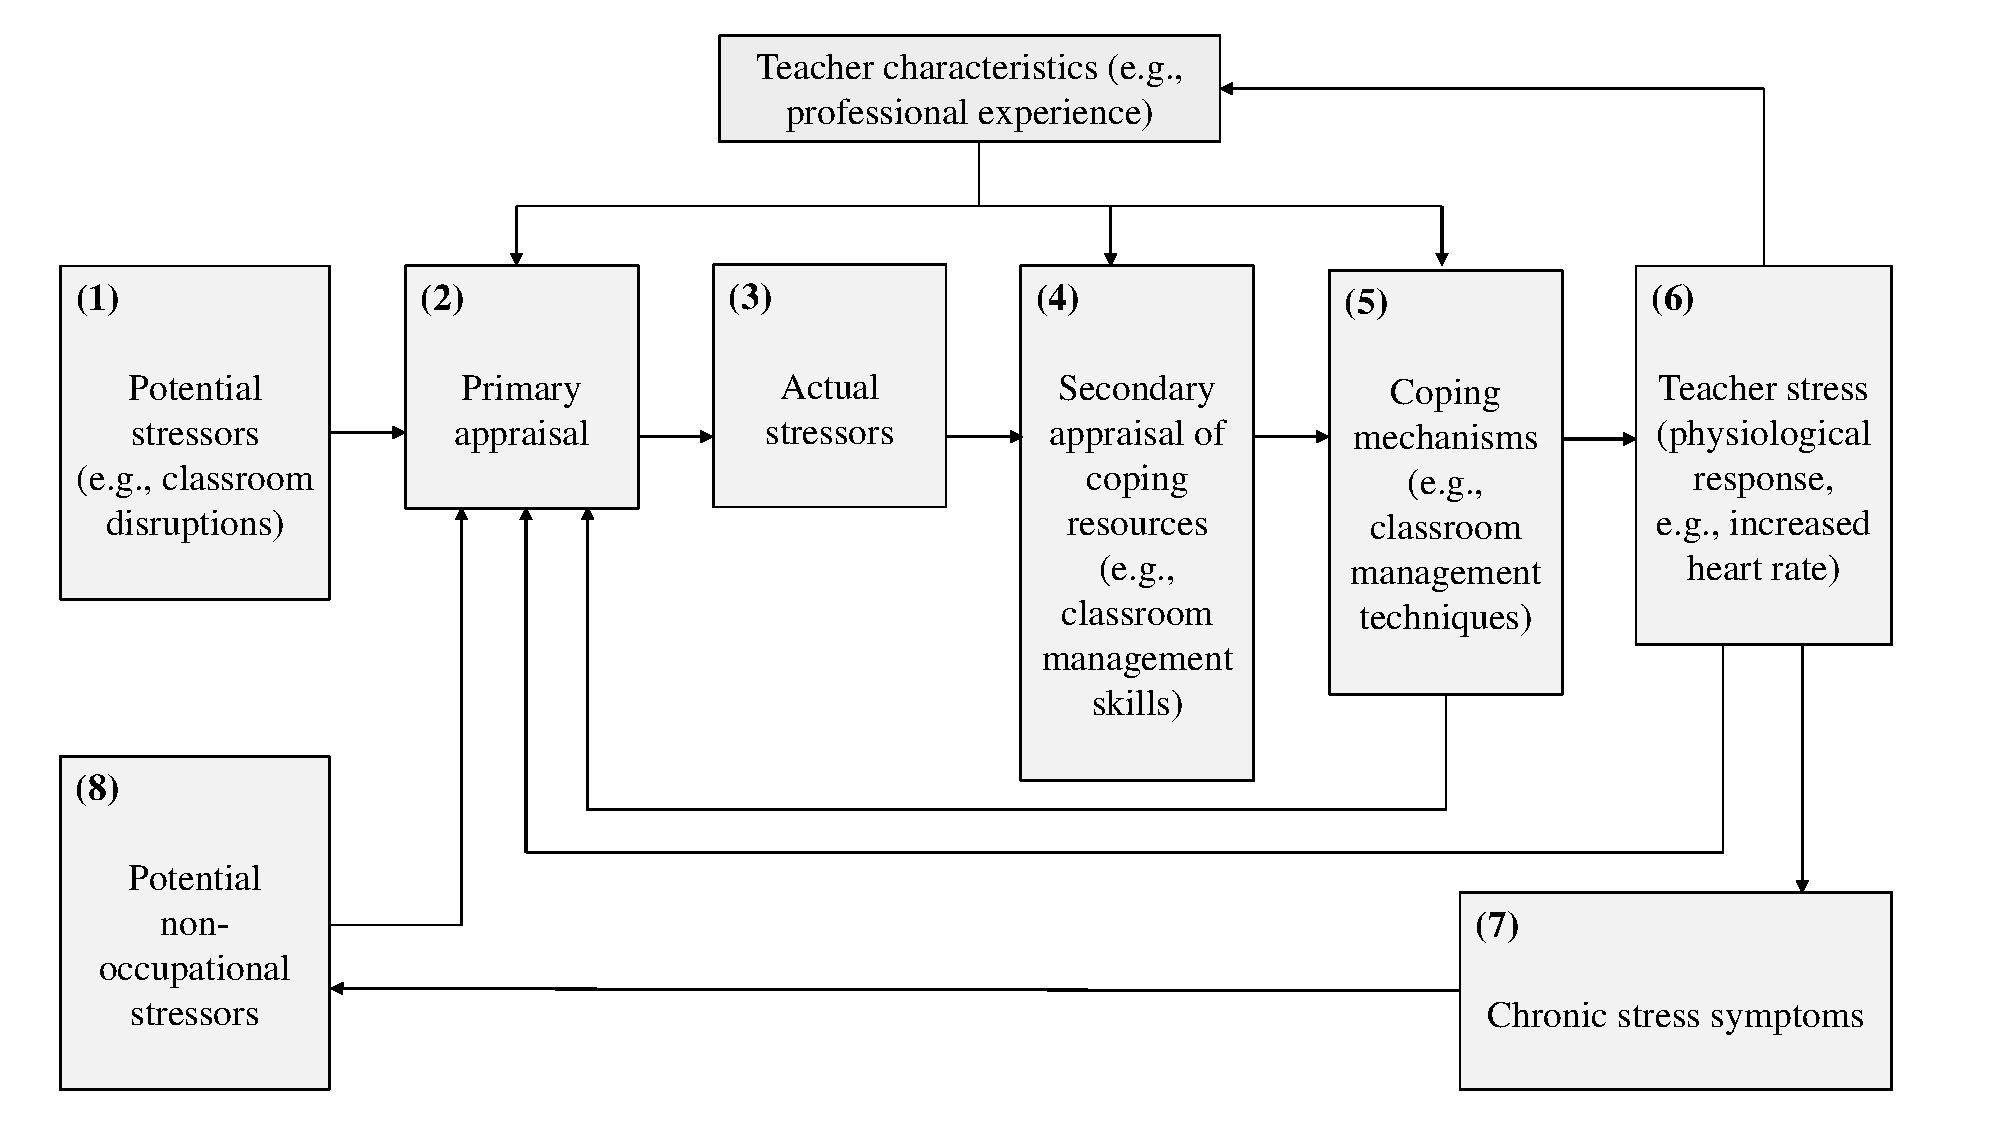
\includegraphics[width=1\textwidth]{images/Model_Teacher_Stress_adapted_new.pdf}
  \caption{A model of teacher stress (adapted from van Dick 2006, p.37, modified by the authors).}
  \label{fig.1}
\end{figure}

\subsection{Present Study}\label{present-study}

The present study aimed to explore the relations between teachers' HR
response, and their subjective appraisals of stress during a
micro-teaching unit, and to relate their self-reported appraisals and
physiological stress responses to their teaching experience. We analyzed
data from in-service and pre-service teachers who participated in a
laboratory study as part of a larger project targeting the development
of classroom management skills. Participants came to the lab
individually and taught a short lesson to a class of three actors (i.e.,
trained student assistants) who performed several typical and possibly
disruptive classroom events. The micro-teaching unit was thus
potentially stressful for the participants. The aims of the present
study were twofold:

\begin{enumerate}
\def\labelenumi{(\arabic{enumi})}
\tightlist
\item
  The first research goal was to investigate whether HR measures
  assessed by a wrist-based fitness tracker were a suitable and
  effective method for mapping teachers' HR over the course of the lab
  study, with a total duration of approximately 2 hours, including
  phases before, during, and after the stressful micro-teaching unit.
\end{enumerate}

Looking at HR measures globally, we expected the participants to show an
initial increase in their HR, followed by a peak during the
micro-teaching unit and a decrease for the remaining phases. In
addition, we examined whether z-standardization of the participants' HR
could serve as a useful method to account for individual differences in
baseline HR: We expected to observe the same trends in both standardized
and non-standardized HR values.

In addition, we selected five representative 10-minute intervals from
the five phases of the lab study (see Fig.\ref{fig.2}) in order to test
the hypotheses that, regarding HR levels, teachers' HR would be the
highest during the micro-teaching unit, compared to all other phases
(Hypothesis 1a), and, regarding HR slopes, that teachers' HR would
increase while they were preparing for teaching (pre-teaching interval),
but decrease in all of the following intervals, i.e.~when they were
habituating to and recovering from the stressful micro-teaching unit
(Hypothesis 1b).

\begin{enumerate}
\def\labelenumi{(\arabic{enumi})}
\setcounter{enumi}{1}
\tightlist
\item
  We further explored whether teaching experience made a difference in
  how teachers' HR reacted to the classroom disruptions. We expected
  more experienced teachers to be less stressed by the classroom events
  (Hypothesis 2a). In addition, we examined the relations between
  teachers' subjective appraisals of the classroom events (specifically,
  the disruptiveness of the events, and their confidence in dealing with
  them) and teachers' HR level, beyond the explanatory power of teaching
  experience. We expected higher HR levels for teachers who felt more
  disrupted, regardless of their teaching experience (Hypothesis 2b),
  and lower HR levels for teachers who felt more confident, regardless
  of teaching experience (Hypothesis 2c). We hypothesized that each of
  the three predictors (\emph{teaching experience, disruption appraisal,
  confidence appraisal}) uniquely contributed to explaining variance in
  teachers' HR levels (Hypothesis 2d). In addition, we exploratively ran
  analogous analyses for the \emph{changes} in HR (i.e., slopes).
\end{enumerate}

\section{Method}\label{method}

\subsection{Participants}\label{participants}

The sample consisted of \(N\) = 84 pre- and in-service teachers from
Germany, who were recruited via personal contacts, email lists, and
flyers. The data of three participants was lost due to failed data
transmission, yielding an analysis sample of \(n_{total}\) = 81
(\(n_{total}\) = 52 women, \(n_{total}\) = 29 men), including 40
pre-service and 41 in-service teachers. Participants had a mean age of
30.95 years (\(SD\) = 10.90; range: 19-60) and an average teaching
experience of 5.64 years (\(SD\) = 9.46; range: 0-37).

\subsection{Setting and Procedure}\label{setting-and-procedure}

The study was carried out following the ethical standards and the
approval of the University's Institutional Review Board. All
participants were informed in detail about the aims of the study prior
to testing. Participation was voluntary, not incentivized, and only took
place after written consent had been given.

Each participant came to the lab for a period of approximately two hours
in total, and each participant underwent the same phases (see
Fig.\ref{fig.2}): In the \emph{pre-teaching phase}, the experimenter
welcomed the participants and helped them put on the fitness tracker.
This was followed by a warm-up session to familiarize the participants
with the laboratory setting and the class. This phase took about 10-15
minutes and participants spent this time mostly standing or slowly
walking around. During the \emph{teaching phase}, the participants held
their self-prepared micro-teaching unit to a class of three trained
actors who performed nine, potentially disruptive, classroom events
(e.g., chatting with a neighbor, heckling, looking at the phone; see
Tab.\ref{tab_a1} in the supplementary material for an overview and
categorization of all events; and Fig.\ref{fig.a2} in the supplementary
material for a depiction of the laboratory setting of the micro-teaching
unit). The topic and class level of the teaching unit could be freely
chosen by the teachers with the only requirement that the unit had to be
an introductory lesson, and had to consist of supervised individual work
and / or frontal teaching. The micro-teaching unit lasted about 15-20
minutes. Participants spent this time mostly standing or slowly walking
around. While teaching, participants wore eye-tracking glasses, and
their lesson was video-recorded. After having completed the
micro-teaching unit, in the \emph{post-teaching phase}, participants
filled in questionnaires for approximately 10-15 minutes: a brief
computer-based survey of sociodemographic data (e.g., teaching
experience, gender, studied school type, studied school subjects,
extracurricular teaching activities), and a short knowledge test that
was irrelevant to the present study. In the \emph{interview phase},
participants engaged in a Stimulated Recall Interview (SRI). During the
SRI, participants sat in front of a computer monitor and watched the
video of their own lesson from the ego perspective, as recorded through
the eye-tracking glasses. The experimenter stopped the video each time
one of the nine classroom events happened, and asked five open-ended,
and three rating questions per event. Two of the rating questions are
relevant to the present study: the disruption and the confidence
appraisal ratings (see Measures). The interview lasted about 45-60
minutes. Finally, in the \emph{end phase}, participants filled in
another questionnaire irrelevant to the present study, which lasted
about 10-15 minutes. \newpage

\begin{wrapfigure}[36]{r}{0.5\textwidth}
  \centering
  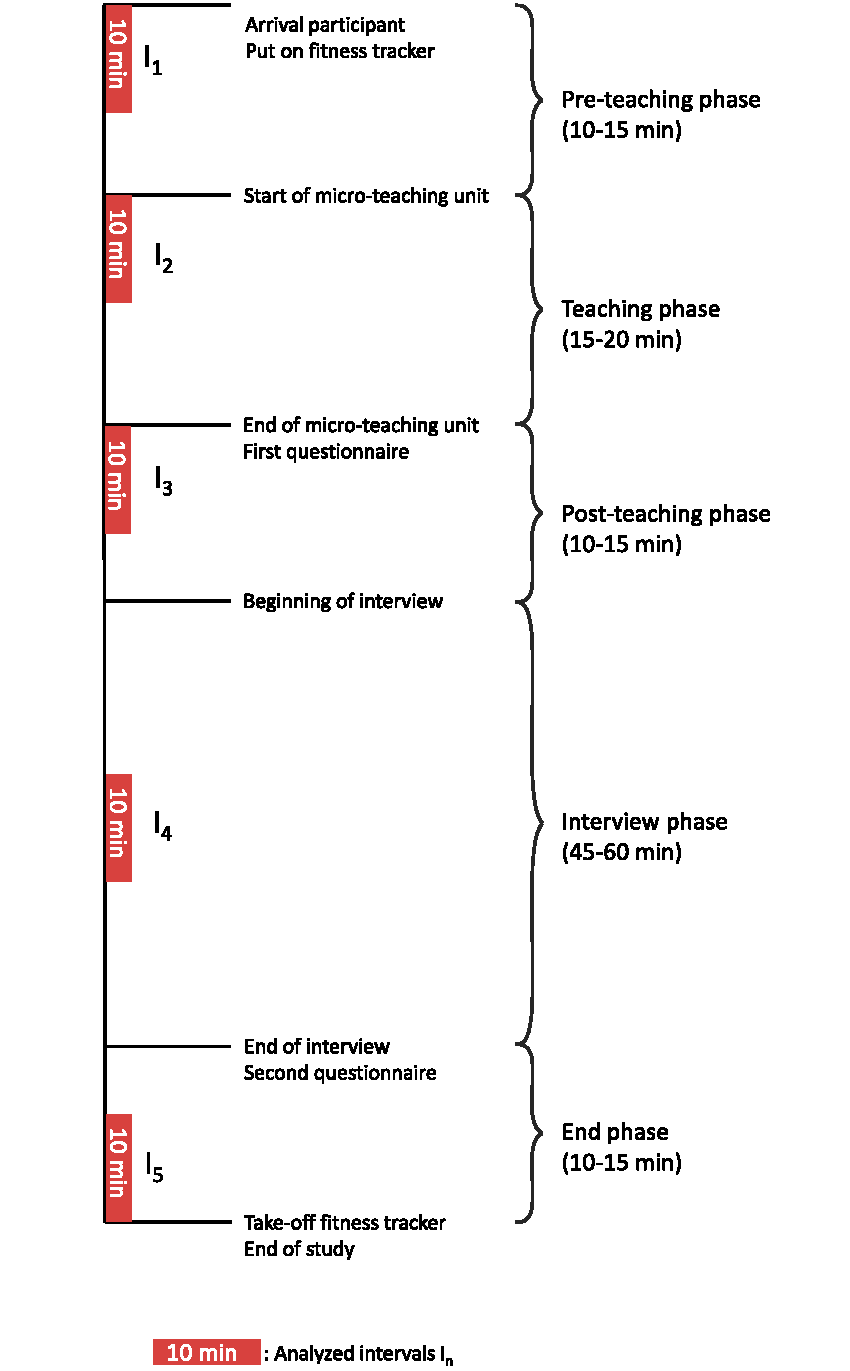
\includegraphics[width=0.5\textwidth]{images/Timeline_smaller.pdf}
  \caption{Procedure of the two-hour-long study consisting of five phases with five representative 10-minute intervals.}
  \label{fig.2}
\end{wrapfigure}

\subsection{Measures}\label{measures}

\subsubsection{Heart Rate Data and Heart Rate
Intervals}\label{heart-rate-data-and-heart-rate-intervals}

To measure teachers' HR, we used the wrist-based fitness tracker Fitbit®
Charge 4. In line with the manufacturer's instructions \citep{fitbitnd},
the device was attached to the participants' nondominant hand, a
finger's width above the wrist bone. The tracker works by flashing green
LEDs hundreds of times per second, using light-sensitive photodiodes to
catch the reflected light, to calculate the volume changes in the
capillaries. From this, the tracker calculated the heart beats per
minute. HR measurements were generated at least every 15
seconds\footnote{The fluctuations in the number of seconds in which the
  HR was measured are due to the participants' movements, meaning that
  the device could not measure the HR every second.}. The raw data
contained the estimated HR in BPM for each time stamp. To account for
individual differences in the baseline HR, we also calculated
z-standardized HR values based on individual means, i.e., at the subject
level of \(n\) = 81 participants (standardized HR).

Since we aimed to keep measurement intervals comparable between study
phases, we aggregated HR over a representative 10-minute interval within
each phase (cf.~Fig.\ref{fig.2}). Previous research has indicated that
10-minute intervals are a useful duration for analyzing PPG data
\citep{lu2008can}. The intervals were selected based on the following
rules: The \emph{pre-teaching interval} (\(I_1\)) comprised the first 10
minutes after the fitness tracker had been put on. The \emph{teaching
interval} (\(I_2\)) started two minutes after the lesson had started.
This interval was of the highest relevance to our study. We explicitly
chose an early 10-minute interval within the teaching phase, as previous
studies revealed that the beginning of a lesson is most demanding and
potentially stressful with regards to teacher-student interaction
\citep{donker2018, claessens2017positive}. The \emph{post-teaching
interval} (\(I_3\)) started immediately after the end of the teaching
unit. The \emph{interview interval} (\(I_4\)) was defined as the mid-10
minutes between the end of the teaching unit and the time point when the
fitness tracker was taken off. All participants were being interviewed
during this interval. The end interval (\(I_5\)) comprised the last 10
minutes before the fitness tracker was taken off.

\subsubsection{Teaching Experience}\label{teaching-experience}

Participants' teaching experience was assessed as a part of their
sociodemographic data. Participants stated their work experience in
years.

\subsubsection{Subjective appraisal of the classroom events and coping
processes}\label{subjective-appraisal-of-the-classroom-events-and-coping-processes}

The subjective disruption and confidence appraisals were assessed during
the SRI on an 11-point rating scale, ranging from 0 (not at all
disrupting/confident) to 10 (extremely disrupting/confident). Ratings
were averaged across the nine classroom events for each participant, as
we were interested in the general stressfulness of the \emph{teaching
phase} for each participant.

\subsection{Data analysis}\label{data-analysis}

We conducted all analyses with R \citep{RStudio2020}. Graphics were
created using ggplot2 \citep{ggplot2}.

To enable visual inspection of HR trends, we displayed smoothed teacher
HR over the course of the recording.\footnote{The curve was smoothed
  using the geom\_smooth() function from the ggplot2 package in R
  \citep{ggplot2} based on the smoothing method LOESS (Locally Estimated
  Scatterplot Smoothing). This method fits a polynomial surface
  determined by one or more numerical predictors, using local fitting.}
We visually compared unstandardized and standardized HR trends over the
two-hour recording period.\footnote{Note that the study exceeded the
  planned duration of two hours for a few participants. To avoid
  distortions when mapping the HR over the course of the study (see
  Fig.\ref{fig.3}), the endpoint was set at two hours for all
  participants, even though data from later time points was used in the
  \emph{end interval} for a few participants.} For all further analyses,
we used standardized rather than unstandardized HR values.

We averaged each person's standardized HR over each of the five selected
intervals\footnote{We used the mean standardized HR instead of the mean
  intercept as we wanted to explain the mean HR of the entire intervals
  and not the HR at the very beginning of the interval (\(x\) = 0).},
resulting in one measure per person per interval. To test Hypothesis 1a,
we initially conducted a one-way ANOVA with repeated measures as an
omnibus test and then tested the mean differences between the
\emph{teaching interval} (\(I_2\)) and the other four intervals by
planned contrasts and inspection of effect size \(d\)
\citep{cohen1988statistical}.

For testing Hypothesis 1b, concerning HR changes within each interval,
we first conducted a linear estimation of the increase or decrease in
standardized HR values over time for each participant. To this end, we
used fixed intercept fixed slope regression models
\citep{gelman2006data} for each interval to estimate intercepts and
linear slopes for each individual, which were then averaged across
individuals.\footnote{Although this procedure does not account for
  nonmonotonic progressions in individual HR, a graphical evaluation
  revealed that the linear estimates corresponded well to the majority
  of the cases (see Fig.\ref{fig.a3} to \ref{fig.a7} in the
  supplementary material).} We tested Hypothesis 1b based on the
unstandardized estimates of mean slopes (one estimate per participant
per interval).

Addressing our second research goal, we ran linear regression analysis
with teaching experience and subjective appraisals as predictors. To
test Hypothesis 2a, we examined the effect of teaching experience on
participants' HR levels (i.e., mean standardized HR) for each of the
five intervals, using linear regression models with teaching experience
as the sole predictor. To test Hypotheses 2b and 2c, we separately
augmented the model by either teachers' disruption appraisal (Hypothesis
2b) or confidence appraisal (Hypothesis 2c) as predictors, while
controlling for teaching experience. To test Hypothesis 2d, we examined
the effects of all three predictors in one regression model.
Furthermore, we repeated these steps to explore the effects of teaching
experience and subjective appraisals on \emph{changes} in teachers' HR
(i.e., mean slopes).\footnote{Please note: HR levels and changes were
  not regressed on the disruption and confidence appraisals in the
  \emph{pre-teaching interval} (\(I_1\)), because the appraised
  classroom events had not yet taken place in that phase.}

\section{Results}\label{results}

\subsection{Mapping teachers' HR over the course of the study
phases}\label{mapping-teachers-hr-over-the-course-of-the-study-phases}

Means, standard deviations, and range of teachers' unstandardized and
standardized HR for the entire study period, and for the five intervals,
are shown in Tab.\ref{tab_1}. Fig.\ref{fig.3} displays the
unstandardized and standardized HR trends, respectively, over the course
of the entire study period. HR initially increased, peaked, and then
decreased, with the unstandardized and standardized HR graphs showing
high similarity. Thus, for all further analyses, we used participants'
standardized HR values.

Fig.\ref{fig.4} shows the distribution of teachers' mean standardized HR
for the five intervals. Repeated measures ANOVA revealed significant
differences in mean standardized HR between intervals,
\(F(4, 400) = 260.62\), \(p < .05\), \(d = 1.60\) (large effect).
Planned contrasts indicated that, as hypothesized (Hypothesis 1a), mean
standardized HR was significantly higher in the \emph{teaching interval}
(\(I_2\)) than in all other intervals, specifically, the
\emph{pre-teaching interval} (\(I_1\); \(t(400) = -10.08\), \(p < .05\),
\(d = 1.034\); large effect), the post-teaching interval (\(I_3\);
\(t(400) = -6.94\), \(p < .05\), \(d = 1.37\); large effect), the
interview interval (\(I_4\); \(t(400) = 15.00\), \(p < .05\),
\(d = 3.29\); large effect), and the end interval (\(I_5\));
\(t(400) = 22.54\), \(p < .05\), \(d = 4.64\); large effect).

Next, we examined HR changes (i.e., mean slopes) within each interval to
test the hypothesis that HR increased during the \emph{pre-teaching
phase} and decreased during all other phases (Hypothesis 1b). The mean
intercepts and mean slopes, complemented by their standard deviations
for each interval, are shown in Tab.\ref{tab_2}. The mean slope of the
\emph{pre-teaching interval} (\(I_1\)) was significantly positive,
indicating an increase in HR, as hypothesized. Further, the mean slopes
of the \emph{teaching interval} (\(I_2\)), \emph{post-teaching interval}
(\(I_3\)), and \emph{interview interval} (\(I_4\)) were significantly
negative, indicating a decrease in HR. For the last interval, the
\emph{end interval} (\(I_5\)), the mean slope was negative, but did not
differ significantly from zero.

\renewcommand{\arraystretch}{1.5}

\begin{table}[ht]
    \centering
    \begin{tabularx}{\textwidth}{lXXXXX}
        \toprule
        Interval & \textit{M} HR & \textit{SD} HR & Min & Max \\
        \midrule
        Overall Course of 2h & 90.09/0.04\footnotemark[12] & 15.76/0.991 & 51/-4.03 & 164/4.56 \\
        Pre-teaching interval (I$_1$) & 96.28/0.48 & 14.11/0.88 & 56/-3.56 & 139/3.24 \\
        Teaching interval (I$_2$) & 100.80/0.85 & 16.23/0.77 & 63/-2.18 & 164/4.37 \\
        Post-teaching interval (I$_3$) & 93.61/0.27 & 14.01/0.76 & 60/-2.17 & 150/3.06 \\
        Interview interval (I$_4$) & 82.32/-0.72 & 11.85/0.74 & 51/-2.51 & 132/4.39 \\
        End interval (I$_5$) & 77.95/-1.07 & 11.14/0.57 & 50\footnotemark[13]/-2.68 & 120/2.96 \\
        \bottomrule
    \end{tabularx}
    \caption{Mean HR (\textit{M}), standard deviations HR (\textit{SD}), and range of teachers’ HR over the course of the entire study and the five intervals (unstandardized in BPM/z-standardized).}
    \label{tab_1}

    
\end{table}
 \footnotetext[12]{Please note that standardized \textit{M} and \textit{SD} of the overall course were not exactly 0 and 1 due to rounding differences.}
 \footnotetext[13]{Deviations of the minimum values in the overall course vs. the \textit{end interval} ($I_5$) are due to data of a few participants who needed more than two hours to finish the study.}

\renewcommand{\arraystretch}{1.5} 

\begin{table}[ht]
    \centering
    \begin{tabularx}{\textwidth}{lXXXXXX}
        \toprule
        Interval  & \multicolumn{2}{c}{\textit{M} (\textit{SD})} & \multicolumn{2}{c}{$p$} \\ & Intercept & Slope & Intercept & Slope \\
        \midrule
        Pre-teaching interval (I$_1$) & 0.052 (0.820) & 0.085 (0.133) & .57 & $< .05$ \\
        Teaching interval (I$_2$) & 1.025 (0.690) & -0.039 (0.108) & $< .05$ & $< .05$ \\
        Post-teaching interval (I$_3$) & 0.549 (0.547) & -0.060 (0.101) & $< .05$ & $< .05$ \\
        Interview interval (I$_4$) & -0.617 (0.614) & -0.022 (0.070) & $< .05$ & $< .05$ \\
        End interval (I$_5$) & -1.004 (0.500) & -0.012 (0.074) & $< .05$ & .14 \\
        \bottomrule
    \end{tabularx}
    \caption{Analysis (\textit{M, SD, p}-values) for the mean intercepts and the mean slopes for the five intervals.}
    \label{tab_2}
\end{table}

\begin{figure}[H]
  \centering
  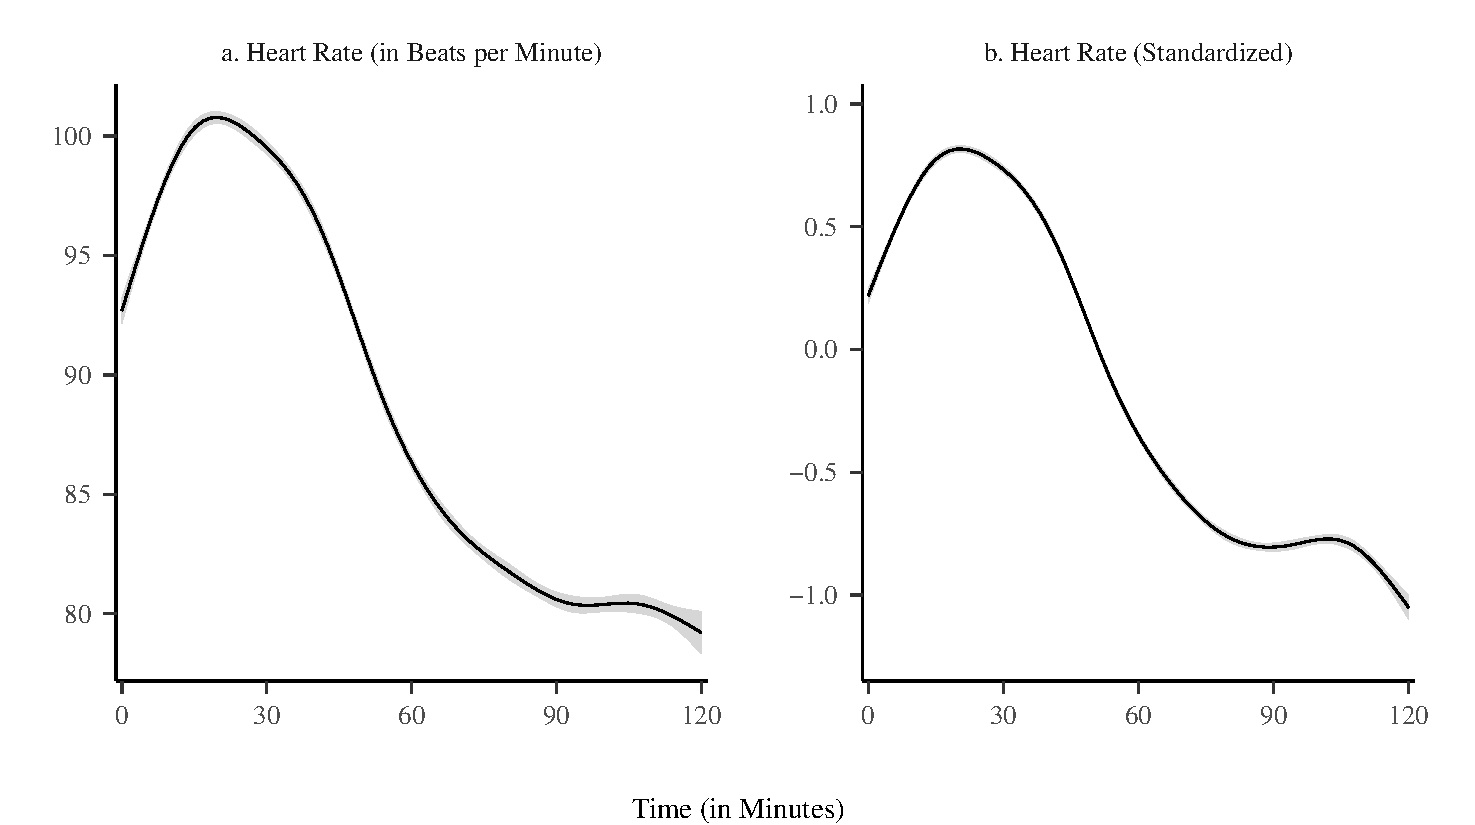
\includegraphics[width=1\textwidth]{plots_publication/loess_plot_std_unstd_new.pdf}
  \caption{Overall course of the HR with the unstandardized HR in BPM shown in Fig.3a. and the z-standardized HR shown in Fig.3b. for the planned 2-hour study.}
  \label{fig.3}
\end{figure}

\begin{figure}[H]
  \centering
  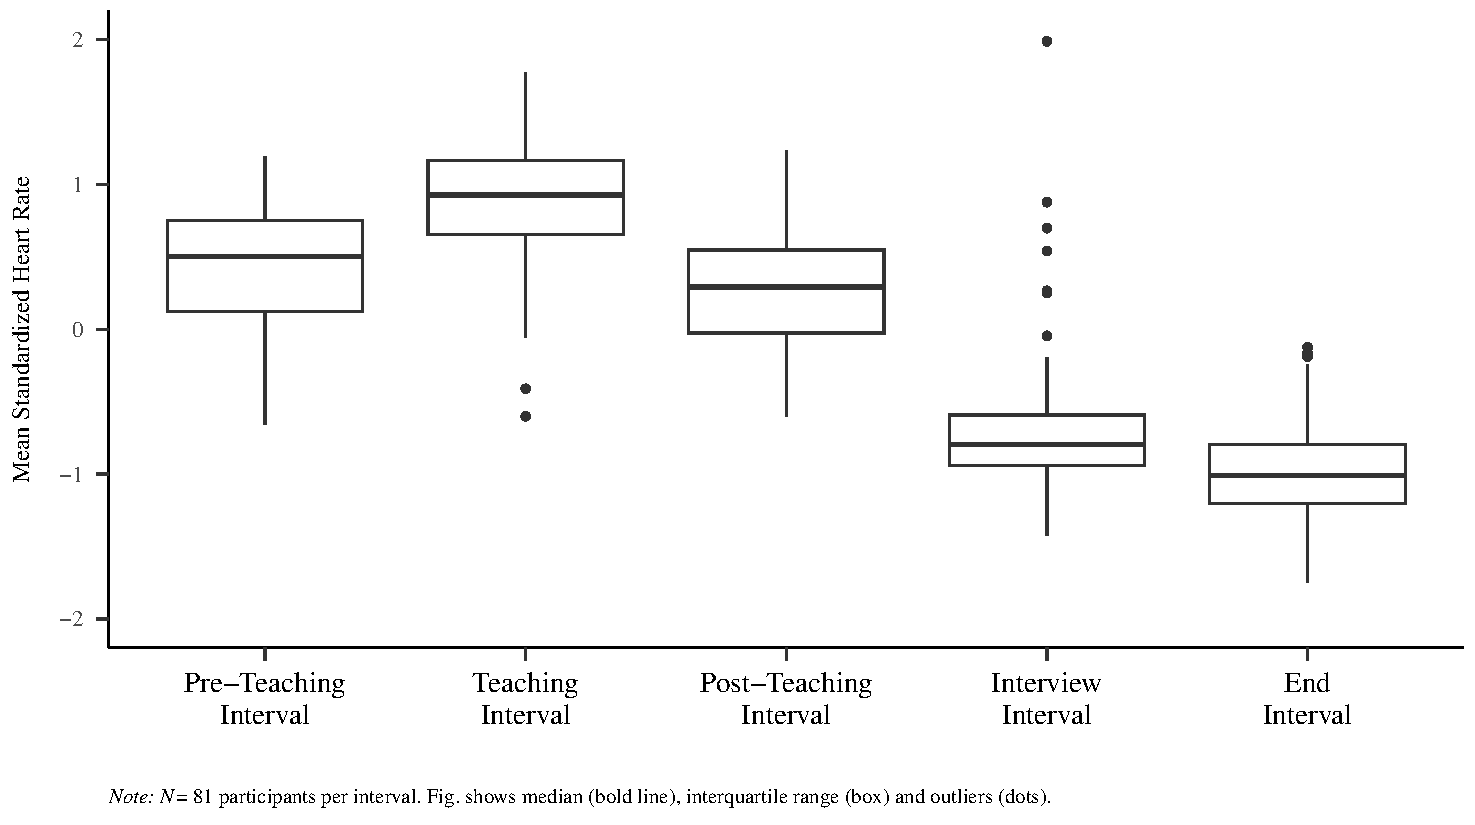
\includegraphics[width=1\textwidth]{plots_publication/box_plot.pdf}
  \caption{Distribution of the standardized heart rate means in the five intervals.}
  \label{fig.4}
\end{figure}

\subsection{Predicting mean standardized HR and mean
slopes}\label{predicting-mean-standardized-hr-and-mean-slopes}

Tab.\ref{tab_3} shows the raw correlations among mean standardized
HR/mean slopes (see Tab.\ref{tab_2} for means and standard deviations),
teaching experience (\(M = 5.64\), \(SD = 9.46\)), disruption appraisal
(\(M = 5.19\), \(SD = 2.87\)), and confidence appraisal (\(M = 7.81\),
\(SD = 1.97\)). With a few notable exceptions, correlations with HR
measures were mostly very small and statistically non-significant
(Tab.\ref{tab_3}). Correlations between teaching experience and
appraisals (not shown in Tab.\ref{tab_3}) were substantial: more
experienced teachers gave lower disruption appraisals (\(r = -.36\)),
and higher confidence appraisals (\(r = .44\)). Moreover, the two
appraisal variables were negatively correlated (\(r = -.37\)).

Tab.\ref{tab_4} shows the results of the regression analyses. Teaching
experience significantly predicted mean standardized HR only in the
\emph{interview interval} (Tab.\ref{tab_4}, \emph{interview interval},
Model 1), indicating a higher mean standardized HR for teachers with
more teaching experience. This relationship is, in fact, in the opposite
direction as predicted by Hypothesis 2a. Neither adding disruption
appraisal (Hypothesis 2b) nor adding confidence appraisal (Hypothesis
2c) increased the amount of explained variance to a statistically
significant extent.

When considering the effects of the three predictors in concert
(Hypothesis 2d), mean standardized HR was significantly predicted only
by disruption appraisal, and only in the \emph{post-teaching interval}
(Tab.\ref{tab_4}, \emph{post-teaching interval}, Model 4), indicating a
higher mean standardized HR for teachers who felt more disrupted by the
classroom events, when controlling for the other variables.

Concerning the explorative investigation of the effects of teaching
experience and subjective appraisals on \emph{changes} (i.e., mean
slopes) in teachers' HR, teaching experience significantly predicted the
mean slope in the \emph{pre-teaching interval} (Tab.\ref{tab_4},
Pre-teaching interval, Model 1), indicating a less steep HR increase in
teachers with more teaching experience. For all other intervals, no
variable had significant predictive value.

\renewcommand{\arraystretch}{1.5}

\begin{table}[h]
    \centering
    \begin{tabularx}{\textwidth}{lccccc}
        \toprule
        Variable & Pre-teaching & Teaching & Post-teaching & Interview & End \\
        & interval & interval & interval & interval & interval \\
        \midrule
        Teaching Experience & $- .17/ - .27^*$ & .11/-.02 & $- .04/-.03$ & $.24^*/-.20$ & .04/.11 \\
        Disruption Appraisal & $- .01/.16$ & $- .20/.08$ & .20/$- .14$ & $- .13/.01$ & .04/.12 \\
        Confidence Appraisal & $- .10/ - .18$ & .06/.09 & .04/$- .03$ & .09/$- .19$ & $- .07/.13$ \\
        \bottomrule \\
          \textit{Note. *} $p < .05$.
    \end{tabularx}
    \caption{Correlations between mean standardized HR/mean slopes and the predictor variables of teaching experience, disruption appraisal, and confidence appraisal for the five intervals.}
    \label{tab_3}
\end{table}

\newpage

\begin{landscape}

\setlength{\LTleft}{0pt}
\setlength{\LTright}{0pt}

\begin{longtable}{@{\extracolsep{\fill}} p{1.8cm} p{1cm} p{1cm} p{1cm} p{1cm} p{1cm} p{1cm} p{1cm} p{1cm} p{1cm} p{1cm} p{1cm} p{1cm} p{1cm} p{1cm} p{1cm} p{1cm} @{}}
    
    \toprule
    & \multicolumn{4}{c}{Model 1} & \multicolumn{4}{c}{Model 2} & \multicolumn{4}{c}{Model 3} & \multicolumn{4}{c}{Model 4} \\
    \cmidrule(lr){2-5} \cmidrule(lr){6-9} \cmidrule(lr){10-13} \cmidrule(lr){14-17}
    Dependent \newline variable: & \multicolumn{16}{c}{Mean standardized HR and mean slopes} \\
    \cmidrule(lr){2-17}
    & \multicolumn{2}{c}{Mean std. HR} & \multicolumn{2}{c}{Mean slopes} & \multicolumn{2}{c}{Mean std. HR} & \multicolumn{2}{c}{Mean slopes} & \multicolumn{2}{c}{Mean std. HR} & \multicolumn{2}{c}{Mean slopes} & \multicolumn{2}{c}{Mean std. HR} & \multicolumn{2}{c}{Mean slopes} \\
    & $\beta$ (SE) & $p$ & $\beta$ (SE) & $p$ & $\beta$ (SE) & $p$ & $\beta$ (SE) & $p$ & $\beta$ (SE) & $p$ & $\beta$ (SE) & $p$ & $\beta$ (SE) & $p$ & $\beta$ (SE) & $p$ \\
    \midrule
    \endfirsthead

    \toprule
    & \multicolumn{4}{c}{Model 1} & \multicolumn{4}{c}{Model 2} & \multicolumn{4}{c}{Model 3} & \multicolumn{4}{c}{Model 4} \\
    \cmidrule(lr){2-5} \cmidrule(lr){6-9} \cmidrule(lr){10-13} \cmidrule(lr){14-17}
    Dependent variable: & \multicolumn{16}{c}{Mean standardized HR and mean slopes} \\
    \cmidrule(lr){2-17}
    & $\beta$ (SE) & $p$ & $\beta$ (SE) & $p$ & $\beta$ (SE) & $p$ & $\beta$ (SE) & $p$ & $\beta$ (SE) & $p$ & $\beta$ (SE) & $p$ & $\beta$ (SE) & $p$ & $\beta$ (SE) & $p$ \\
    \midrule
    \endhead

    \bottomrule
    \multicolumn{17}{c}{{Continued on next page}} \\
    \endfoot

    \bottomrule
    \endlastfoot

    Pre-teaching \newline interval ($I_1$) & & & & & & & & & & & & & & & & \\
    Teaching \newline Experience & \begin{tabular}{@{}c@{}}$-.17$\\$(.005)$\end{tabular} & $.12$ & \begin{tabular}{@{}c@{}}$-.27^*$\\$(.002)$\end{tabular} & $<.05$ & & & & & & & & & & & & \\
    R\textsuperscript{2} & $.030$ & & $.071$ & & & & & & & & & & & & & \\
    \midrule
    Teaching \newline interval ($I_2$) & & & & & & & & & & & & & & & & \\
    Teaching \newline Experience & \begin{tabular}{@{}c@{}}$.11$\\$(.002)$\end{tabular} & $.34$ & \begin{tabular}{@{}c@{}}$-.02$\\$(.001)$\end{tabular} & $.83$ & \begin{tabular}{@{}c@{}}$.04$\\$(.005)$\end{tabular} & $.73$ & \begin{tabular}{@{}c@{}}$.01$\\$(.001)$\end{tabular} & $.96$ & \begin{tabular}{@{}c@{}}$.10$\\$(.006)$\end{tabular} & $.42$ & \begin{tabular}{@{}c@{}}$-.08$\\$(.001)$\end{tabular} & $.54$ & \begin{tabular}{@{}c@{}}$.05$\\$(.006)$\end{tabular} & $.67$ & \begin{tabular}{@{}c@{}}$-.05$\\$(.001)$\end{tabular} & $.72$ \\
    Disruption \newline Appraisal & \begin{tabular}{@{}c@{}}$-.18$\\$(.041)$\end{tabular} & $.13$ & \begin{tabular}{@{}c@{}}$.08$\\$(.010)$\end{tabular} & $.50$ & \begin{tabular}{@{}c@{}}$-.19$\\$(.042)$\end{tabular} & $.13$ & \begin{tabular}{@{}c@{}}$.12$\\$(.010)$\end{tabular} & $.34$ \\
    Confidence \newline Appraisal & \begin{tabular}{@{}c@{}}$.01$\\$(.046)$\end{tabular} & $.92$ & \begin{tabular}{@{}c@{}}$.12$\\$(.011)$\end{tabular} & $.34$ & \begin{tabular}{@{}c@{}}$-.04$\\$(.047)$\end{tabular} & $.76$ & \begin{tabular}{@{}c@{}}$.15$\\$(.012)$\end{tabular} & $.24$ \\
    R\textsuperscript{2} & $.012$ & & $.000$ & & $.040$ & & $.015$ & & $.012$ & & $.010$ & & $.042$ & & $.031$ \\
    $\Delta$ R\textsuperscript{2} & & & $.028$ & & $.015$ & & $.000$ & & $.010$ & & $.030$ & & $.031$ \\
    \midrule
    Post-teaching \newline interval ($I_3$) & & & & & & & & & & & & & & & & \\
    Teaching \newline Experience & \begin{tabular}{@{}c@{}}$-.04$\\$(.005)$\end{tabular} & $.70$ & \begin{tabular}{@{}c@{}}$-.03$\\$(.001)$\end{tabular} & $.80$ & \begin{tabular}{@{}c@{}}$.04$\\$(.005)$\end{tabular} & $.76$ & \begin{tabular}{@{}c@{}}$-.09$\\$(.001)$\end{tabular} & $.44$ & \begin{tabular}{@{}c@{}}$-.08$\\$(.006)$\end{tabular} & $.55$ & \begin{tabular}{@{}c@{}}$-.02$\\$(.001)$\end{tabular} & $.89$ & \begin{tabular}{@{}c@{}}$-.01$\\$(.006)$\end{tabular} & $.91$ & \begin{tabular}{@{}c@{}}$-.07$\\$(.001)$\end{tabular} & $.61$ \\
    Disruption \newline Appraisal & \begin{tabular}{@{}c@{}}$.22$\\$(.040)$\end{tabular} & $.07$ & \begin{tabular}{@{}c@{}}$-.18$\\$(.009)$\end{tabular} & $.14$ & \begin{tabular}{@{}c@{}}$.25^*$\\$(.041)$\end{tabular} & $<.05$ & \begin{tabular}{@{}c@{}}$-.20$\\$(.010)$\end{tabular} & $.12$ \\
    Confidence \newline Appraisal & \begin{tabular}{@{}c@{}}$.08$\\$(.045)$\end{tabular} & $.55$ & \begin{tabular}{@{}c@{}}$-.03$\\$(.011)$\end{tabular} & $.83$ & \begin{tabular}{@{}c@{}}$.14$\\$(.046)$\end{tabular} & $.27$ & \begin{tabular}{@{}c@{}}$-.08$\\$(.011)$\end{tabular} & $.54$ \\
    R\textsuperscript{2} & $.002$ & & $.001$ & & $.043$ & & $.020$ & & $.006$ & & $.002$ & & $.058$ & & $.023$ \\
    $\Delta$ R\textsuperscript{2} & & & $.041$ & & $.019$ & & $.004$ & & $.001$ & & $.056$ & & $.022$ \\
    \midrule
    Interview \newline interval ($I_4$) & & & & & & & & & & & & & & & & \\
    Teaching \newline Experience & \begin{tabular}{@{}c@{}}$.24^*$\\$(.006)$\end{tabular} & $<.05$ & \begin{tabular}{@{}c@{}}$-.20$\\$(.001)$\end{tabular} & $.07$ & \begin{tabular}{@{}c@{}}$.22$\\$(.006)$\end{tabular} & $.06$ & \begin{tabular}{@{}c@{}}$-.23$\\$(.001)$\end{tabular} & $.06$ & \begin{tabular}{@{}c@{}}$.25^*$\\$(.006)$\end{tabular} & $<.05$ & \begin{tabular}{@{}c@{}}$-.14$\\$(.001)$\end{tabular} & $.25$ & \begin{tabular}{@{}c@{}}$.23$\\$(.007)$\end{tabular} & $.07$ & \begin{tabular}{@{}c@{}}$-.17$\\$(.001)$\end{tabular} & $.18$ \\
    Disruption \newline Appraisal & \begin{tabular}{@{}c@{}}$-.05$\\$(.045)$\end{tabular} & $.66$ & \begin{tabular}{@{}c@{}}$-.08$\\$(.006)$\end{tabular} & $.52$ & \begin{tabular}{@{}c@{}}$-.06$\\$(.047)$\end{tabular} & $.61$ & \begin{tabular}{@{}c@{}}$-.12$\\$(.007)$\end{tabular} & $.34$ \\
    Confidence \newline Appraisal & \begin{tabular}{@{}c@{}}$-.02$\\$(.050)$\end{tabular} & $.85$ & \begin{tabular}{@{}c@{}}$-.13$\\$(.007)$\end{tabular} & $.29$ & \begin{tabular}{@{}c@{}}$-.04$\\$(.052)$\end{tabular} & $.76$ & \begin{tabular}{@{}c@{}}$-.16$\\$(.007)$\end{tabular} & $.20$ \\
    R\textsuperscript{2} & $.058$ & & $.040$ & & $.060$ & & $.050$ & & $.058$ & & $.054$ & & $.061$ & & $.069$ \\
    $\Delta$ R\textsuperscript{2} & & & $.002$ & & $.010$ & & $.000$ & & $.014$ & & $.003$ & & $.029$ \\
    \midrule
    End \newline interval ($I_5$) & & & & & & & & & & & & & & & & \\
    Teaching \newline Experience & \begin{tabular}{@{}c@{}}$.04$\\$(.004)$\end{tabular} & $.70$ & \begin{tabular}{@{}c@{}}$.11$\\$(.001)$\end{tabular} & $.32$ & \begin{tabular}{@{}c@{}}$.07$\\$(.005)$\end{tabular} & $.58$ & \begin{tabular}{@{}c@{}}$.18$\\$(.001)$\end{tabular} & $.13$ & \begin{tabular}{@{}c@{}}$.09$\\$(.005)$\end{tabular} & $.46$ & \begin{tabular}{@{}c@{}}$.07$\\$(.001)$\end{tabular} & $.58$ & \begin{tabular}{@{}c@{}}$.10$\\$(.005)$\end{tabular} & $.43$ & \begin{tabular}{@{}c@{}}$.12$\\$(.001)$\end{tabular} & $.33$ \\
    Disruption \newline Appraisal & \begin{tabular}{@{}c@{}}$.06$\\$(.035)$\end{tabular} & $.60$ & \begin{tabular}{@{}c@{}}$.19$\\$(.007)$\end{tabular} & $.12$ & \begin{tabular}{@{}c@{}}$.04$\\$(.037)$\end{tabular} & $.76$ & \begin{tabular}{@{}c@{}}$.23$\\$(.007)$\end{tabular} & $.07$ \\
    Confidence \newline Appraisal & \begin{tabular}{@{}c@{}}$-.11$\\$(.039)$\end{tabular} & $.38$ & \begin{tabular}{@{}c@{}}$.10$\\$(.008)$\end{tabular} & $.43$ & \begin{tabular}{@{}c@{}}$-.10$\\$(.041)$\end{tabular} & $.44$ & \begin{tabular}{@{}c@{}}$.16$\\$(.008)$\end{tabular} & $.22$ \\
    R\textsuperscript{2} & $.002$ & & $.013$ & & $.005$ & & $.053$ & & $.012$ & & $.025$ & & $.013$ & & $.078$ \\
    $\Delta$ R\textsuperscript{2} & & & $.003$ & & $.040$ & & $.010$ & & $.012$ & & $.011$ & & $.065$ \\
    \label{tab_4}
\end{longtable}
    \captionof{table}{Standardized regression coefficients of mean standardized heart rate and mean slopes predicted by teaching experience, disruption appraisal, and confidence appraisal for the five intervals.}
\begin{tablenotes}
\footnotesize
\item \textit{Note.} In Model 1, mean standardized HR and mean slopes were predicted only by teaching experience. In Model 2, solely disruption appraisal was added to teaching experience as a predictor. In Model 3, solely confidence appraisal was added to teaching experience as a predictor. In Model 4, all three predictors were considered in concert. * $p < .05$.
\end{tablenotes}
\end{landscape}

\section{Discussion}\label{discussion}

\subsection{Key findings}\label{key-findings}

Overall, our findings indicate that wrist-worn fitness trackers are a
useful tool for tracking teachers' HR and identifying stressful periods
during teaching. Using HR data from a commercially available and
relatively low-cost Fitbit® fitness tracker, we were able to map
teachers' HR before, during, and after a stressful micro-teaching unit,
with HR increasing in preparation for teaching, peaking during the
teaching phase, and decreasing afterward.

These findings are in line with prior studies showing that teachers' HR
varies depending on their activities and encountered stressors with
increases during phases where teachers are in an exposed position
\citep{sperka1995, scheuch1997psychophysische, donker2018, junker2021},
as well as with findings showing how HR changes align with activating
events and stress-inducing tasks \citep{Darnell2019, chalmers2021}.

Building on the model of teacher stress (\citet{kyriacou1978}, see
Fig.\ref{fig.2}), we had hypothesized that more experienced teachers,
with better classroom management skills at their disposal, experience
less physiological stress when dealing with classroom disruptions.
Contrary to our expectations, we found no buffering effect of teaching
experience on teachers' HR, i.e., more experienced teachers did not show
lower mean standardized HR during the stressful teaching phase than less
experienced teachers. Rather, at least descriptively, we observed the
opposite trend. There are several possible explanations for this
finding. First, teaching experience is inherently confounded with age
(the two variables correlated at \(r = .94\) in our sample), and age has
been shown to affect indicators of cardiovascular reactivity in various
ways \citep{uchino2010older}. However, to avoid this kind of confounding
influence, we had used not raw BPM but rather standardized mean HR for
all our analyses, thus controlling at least for inter-individual
differences in mean HR. Second, as research on teacher
professionalization has repeatedly shown, professional experience is not
a guarantee for higher professional knowledge and skills
\citep{kirschner2016professionswissen}. Rather, honing skills from
professional experience necessitates a deliberate practice of choosing
to improve, learning through experience, and integrating new knowledge
into future performances \citep{dunn1999deliberate}. Thus, rather than
professional experience alone, more direct assessments of classroom
management skills, such as objective behavior-based tests, would be a
better indicator of expertise that future studies could explore.
Finally, and most importantly, the highly controlled teaching situation
that we created in the lab might not have provided sufficient
resemblance to the expert teachers' working conditions to let them
effectively use their coping resources. In other words, since the
situation was unfamiliar to both experienced and unexperienced teachers,
their stress levels might have been more similar than they would have
been in a more authentic classroom setting.

While we did not find a buffering effect of teaching experience on mean
HR during teaching, we did, however, find a less steep HR increase in
more experienced, compared to less experienced teachers during the
\emph{pre-teaching phase} (\(\beta = -.27\)), i.e., in preparation for
the micro-teaching unit. This finding supports the idea that, even
though teaching experience guarantees neither superior expertise nor
stress resistance, the habits and routines formed by experienced
teachers may at least lead to lower arousal levels (e.g., experienced as
feeling less nervous and tense) when they anticipate potentially
stressful teaching situations.

An interesting observation beyond our hypotheses was that teaching
experience was predictive of HR differences, not during teaching, but in
the \emph{interview phase}: compared to less experienced teachers, more
experienced teachers showed a higher mean standardized HR
(\(\beta = .24\)) and, thus, probably experienced higher levels of
physiological stress during the SRI. One possible explanation for this
finding could again be the higher age of the more experienced teachers,
along with slower recovery from stress in older teachers. For instance,
\citet{ritvanen2006responses} observed that, compared to their younger
colleagues, older teachers did not experience a decrease in their HR
during periods of low stress levels, from which they concluded that
recovery from stress was insufficient in the older teachers
\citep{ritvanen2006responses}. Alternatively, the finding could also be
attributed to the fact that less experienced teachers, due to their
ongoing or only recently concluded training, may have been more
accustomed to reflecting on their work and receiving feedback as was the
case during the SRI, whereas, these activities were less routine and
possibly more face-threatening for experienced teachers. Therefore, it
is possible that more experienced teachers found the interview itself to
be more stressful and therefore showed a higher mean standardized HR
during this phase.

With regards to the predictive power of teachers' subjective appraisals
of the classroom disruption during teaching, we, first of all, have to
conclude that our hypotheses were not supported, as neither confidence
appraisal nor disruptiveness appraisal showed any notable correlations
with teachers' mean standardized HR or any explanatory power over and
beyond teaching experience. Possibly, teachers' self-reported
appraisals, and their actual physiological stress responses, tap into
quite different phenomena, or at least, quite different aspects of the
multifaceted stress response \citep{kyriacou1978}. In addition, while HR
was assessed online during teaching, self-reported appraisals were given
in retrospect during the SRI, and may be subject to biased (e.g.,
self-serving) reporting or simply an inability to recall ones immediate
stress reactions.

On the other hand, when controlling for all other factors, teachers who
reported to have perceived the events as more disruptive showed a higher
HR (\(\beta = .25\)) in the phase immediately following the
micro-teaching unit. This finding would be consistent with the idea that
differences in mean HR, as an indicator of the physiological stress
response, can be linked to the cognitive appraisal of stressors.

\subsection{Limitations and future
directions}\label{limitations-and-future-directions}

While the laboratory setting of the study allowed for a controlled
implementation of stressors and high internal validity, it was not an
authentic classroom environment, raising questions about its external
validity. Most importantly, the teacher and their students did not have
a shared history, and only a very thin basis for establishing a positive
teacher-student relationship, which is a core characteristic of
effective classroom management \citep{ruedi2014, beaty2010}. In
addition, the micro-teaching unit was only about 15 minutes long, and
thus much shorter than a regular school lesson, providing less
opportunities for experienced teachers to build up an engaging lesson.
Finally, student behavior was scripted, with classroom disruptions
following the experimental schedule, irrelevant of the behavior of the
teacher. Thus, the setting may have masked effects of teaching
experience by providing too little opportunities of experienced teachers
to demonstrate their true classroom management skills, in particular
regarding the prevention of disruptions. In subsequent studies, it would
therefore be insightful to assess teachers' HR in more authentic
classroom settings over a longer period of time (e.g., days, weeks, or
even months). Extended observation of teachers' HR in authentic
classroom settings could reveal how factors such as student behavior,
teaching methods, or organizational and administrative demands
contribute to fluctuations in physiological arousal, uncovering insights
into the sustained physiological demands of teaching that short-term
studies may overlook. Finally, linking actual teacher behavior to
potential stressors (e.g., classroom disruptions, noise level, etc.)
would offer insights into teacher coping strategies and their links with
physiological indicators of stress.

Another limitation concerns the assessment of teachers' HR. While our
results demonstrate the usefulness of drawing upon easily available HR
data from ubiquitous, low-cost, un-intrusive fitness trackers to
estimate teacher stress, there also are shortcomings of this type of
assessment. First, while fitness trackers typically yield HR data, heart
rate variability (HRV) has been demonstrated to be an even more accurate
indicator of stress \citep{wettstein2020ambulatory}. While standard
fitness trackers did not provide this measure at the time of our data
collection, more recent products do offer this function. Thus, future
studies might consider assessing HRV instead of HR. Second, we did not
record participants' resting HR, which is generally considered an
important baseline for determining inter- and intrapersonal differences
in cardiovascular health and reactivity
\citep{nanchen2018, heneghan2019}. A clean baseline HR requires a
resting phase without physical movement or emotional stress, ideally
fifteen minutes before the beginning of the activity, which is very
difficult to achieve in practice \citep{sammito2015guideline}, e.g.,
when assessing teacher HR before and during teaching. Thus, our study
explored the possibility of substituting baseline HR measurement via
z-standardization within participants. As a result, the absolute
standardized values of each participant must always be interpreted in
the context of the standardization sample, and thus are less
interpretable than individual BPM values together with a baseline HR.
However, for statistical analyses based on the whole sample, the
standardization fulfills the aim of controlling for differences in
individual HR due to, for example, age-related differences. Finally,
depending on the brand and model of fitness trackers used, the precision
of the HR measurement varies. Research on the reliability of our
deployed Fitbit® device has proven that this brand is generally accurate
in controlled settings and for moderate activity levels
\citep{wallen2016accuracy, hajj2023, fuller2020, jo2016}, as in our
study. For example, the Fitbit® fitness tracker has previously shown
good HR measurement accuracy during resting phases
\citep{jo2016, muggeridge2021measurement} and for activities such as
walking, jogging, and running \citep{hajj2023}. At higher exercise
intensities such as cycling, the Fitbit® tracker may underestimate HR
\citep{thomson2019heart, montoye2017comparative, jo2016, jachymek2021}
but is still within an acceptable range according to systematic reviews
\citep{chevance2022accuracy}. Nevertheless, \citet{gagnon2022} stressed
that Fitbit® trackers cannot replace ECG when precision is paramount.
Despite these considerations, the Fitbit® model appears suitable for our
study purposes, as physical strain was moderate.

Furthermore, while we assessed teachers' appraisals of the stressful
classroom disruptions using a SRI in which they could review the exact
situation, these appraisal ratings were still post-hoc self-reports,
which limits the interpretation of our results. One of the main issues
with post-hoc self-reports is that they rely on the teachers' memories
and subjective interpretations of past events, which may be prone to
various biases such as social desirability \citep{razavi2001self} or
recall errors \citep{van2016accuracy}. Moreover, stress is not a fixed
or stable construct; it is a dynamic, constantly evolving affective
response that can vary depending on context, individual disposition, and
prior experiences, making it particularly challenging to pinpoint valid
and reliable process markers for how individuals appraise stress in
real-time \citep{lazarus1990theory}. While SRIs provide a more detailed
and reflective understanding of the stressor in question, the delayed
nature of the response makes it difficult to capture the immediate,
in-the-moment appraisal that occurs when the stressful event actually
takes place.

\subsection{Hands-on advice for using wrist-worn fitness trackers for
research}\label{hands-on-advice-for-using-wrist-worn-fitness-trackers-for-research}

For researchers aiming to use fitness trackers to collect data, there
are practical aspects to consider concerning the design, data
collection, and data analysis phases of research projects \citep[for an
additional overview, see][]{nelson2020guidelines}:

\begin{enumerate}
\def\labelenumi{\arabic{enumi})}
\tightlist
\item
  Choosing a suitable model:
\end{enumerate}

Before data collection, researchers need to decide which model of
fitness tracker best suits their research question. One important point
to consider is whether the study will be conducted in the laboratory, in
a clinical environment, or under real-world conditions. Conventional
fitness trackers should not be used if the focus is on measurement
accuracy, such as in medical contexts, as they cannot replace the
accuracy of ECG measurements \citep{gagnon2022}. Moreover, researchers
should consider that measurement accuracy also depends on the intensity
of the movements performed by the participants during data collection.
Fitbit® fitness trackers, for example, underestimate HR at higher
exercise intensities such as cycling
\citep{thomson2019heart, montoye2017comparative, jo2016, jachymek2021}.
For reference, the systematic review by \citet{fuller2020} provides a
detailed overview of studies that used wrist-worn fitness trackers
between 2000 and 2019 and discusses their validity and reliability.
Another point to consider is the price, which at the time of writing
ranged between €30 for the cheapest models and up to €1.700 for medical
wristbands. Currently, models assessing HRV in addition to HR are
becoming more and more affordable and widespread. Still, Fitbit® fitness
trackers might be a good choice for teams operating with moderate
budgets or if larger groups of participants need to be tracked at the
same time. Further, before conducting any study, it should be considered
that the data collected with fitness trackers is health data, and
therefore very sensitive. Researchers have to ensure that their chosen
model of fitness tracker allows them to collect and store data in line
with relevant ethical and legal requirements, for example, guaranteeing
participants' anonymity and secure data storage.

\begin{enumerate}
\def\labelenumi{\arabic{enumi})}
\setcounter{enumi}{1}
\tightlist
\item
  Operating the fitness tracker:
\end{enumerate}

In planning the operation of their chosen model of fitness tracker,
researchers need to specify the circumference and attachment of the
wrist band and the placement of the fitness tracker on participants. In
particular, researchers conducting studies with children should take
into account their smaller wrist size. When putting on a fitness
tracker, attention must also be paid to whether it is attached to the
dominant or non-dominant wrist, as this can influence HR measurements.
Different models of fitness trackers need to be placed differently and
in line with the manufacturer's instructions. It is also important to
check that the battery is fully charged each time, that the latest
software version is loaded, and that the fitness tracker has been
synchronized before recording data to avoid unnecessary loss of data.
Finally, if researchers want to accurately investigate parameters during
specific time intervals, such as HR during lessons versus breaks, it is
crucial to synchronize the fitness tracker with other time-keeping
devices, such as watches. This synchronization allows researchers to
precisely determine the onset and offset of particular activities or
intervals of interest. By aligning the recorded data with specific time
frames, researchers can ensure that the physiological measurements, such
as HR, are accurately associated with the corresponding periods of
interest. This process enhances the validity and reliability of the data
analysis, enabling a more precise examination of variations in
physiological responses across different time intervals.

\begin{enumerate}
\def\labelenumi{\arabic{enumi})}
\setcounter{enumi}{2}
\tightlist
\item
  Extracting and analyzing fitness tracker data:
\end{enumerate}

As far as the procedure for processing the data is concerned,
researchers should ensure that the raw data of the physiological
measurements are available for further analysis. For the Fitbit® HR
measurements, for example, the raw data can be downloaded from a website
in the form of .csv files. However, these must be downloaded as soon as
possible after data collection, as some platforms automatically delete
or archive older data files after a certain period due to policies
regarding data storage and retention. This can result in loss of access
to critical data. Additionally, ensuring that data is collected at the
intended sampling rate is crucial for accurate analysis. For instance,
while our fitness tracker was designed to record HR every 1-5 seconds,
we occasionally observed recordings only every 15 seconds, possibly due
to participant movement and tracker placement.

\subsection{Conclusion}\label{conclusion}

This study investigated whether HR data collected from teacher-worn
fitness trackers are suitable for exploring links between HR, subjective
stressor appraisal, and individual teaching experience, to achieve a
more profound comprehension of teacher stress. Results suggest that the
widespread availability of HR data from wearable fitness trackers,
moving ``from heartbeat to data'', presents opportunities both to
teachers for self-monitoring stress levels, and to researchers for
assessing physiological indicators of stress. For example, using fitness
trackers could enable teachers to strengthen their self-awareness in
stressful situations and allow for early self-intervention such as
mindfulness techniques (e.g., deep breathing or body scans;
\citet{agyapong2023interventions}). Integrating fitness trackers into
teacher training and everyday practice could offer an affordable and
practical method for assessing and managing teacher stress. In teacher
training as well as in research, triangulating data from fitness
trackers, lesson videos, and interviews could provide teachers with
insights into their own stress management, and foster the implementation
of effective stress and classroom management strategies. Taken together,
our findings cater to \citet{wettstein2021} call for the use of
ambulatory assessment methods, particularly in the context of classroom
disruptions, for gaining a deeper understanding of teacher stress and
its impact on both psychological and physiological variables.

In summary, our study contributes to the understanding of stress in
educational settings and underscores the potential of wearable fitness
trackers in advancing research on teacher well-being. By harnessing the
power of wearable technology, we can provide teachers with the tools
needed to better understand and manage their stress, ultimately
enhancing their overall well-being.

\newpage

\appendix
\section*{Appendix}

\setcounter{figure}{0}  % Reset figure numbering

\setcounter{table}{0}

\renewcommand{\thefigure}{A\arabic{figure}}  % Figures labeled A1, A2, etc.

\renewcommand{\thetable}{A\arabic{table}}

\renewcommand{\arraystretch}{1.5}

\begin{table}[ht]
    \centering
    \begin{tabularx}{\textwidth}{XXX}
        \toprule
        Verbal disruptions & Physical disruptions & Lack of eagerness to learn \\
        \midrule
        Heckling & Clicking pen & Looking at phone \\
        Chatting & Snipping hands & Drawing \\
        Whispering & Drumming hands & Head on table \\
        \bottomrule
    \end{tabularx}
    \caption{Classification of nine, typical classroom disruptions according to \cite{lohmann2003schulern} performed in the micro-teaching unit by actors.}
    \label{tab_a1}
\end{table}

\begin{figure}[htbp]
  \centering
  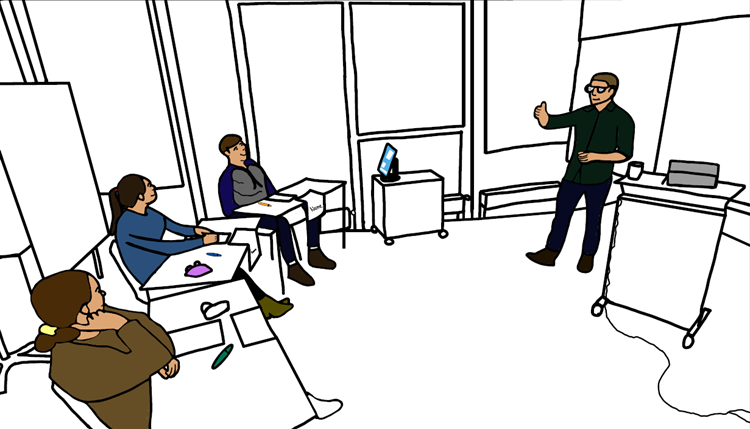
\includegraphics[width=0.45\textwidth]{appendix_figure1.png}
  \caption*{\textit{Note.} The setting included three actors as the class (left) and a teacher (participant, right).}
  \caption{Laboratory setting of the micro-teaching unit.}
  \label{fig.a1}
\end{figure}

\begin{figure}[htbp]
  \centering
  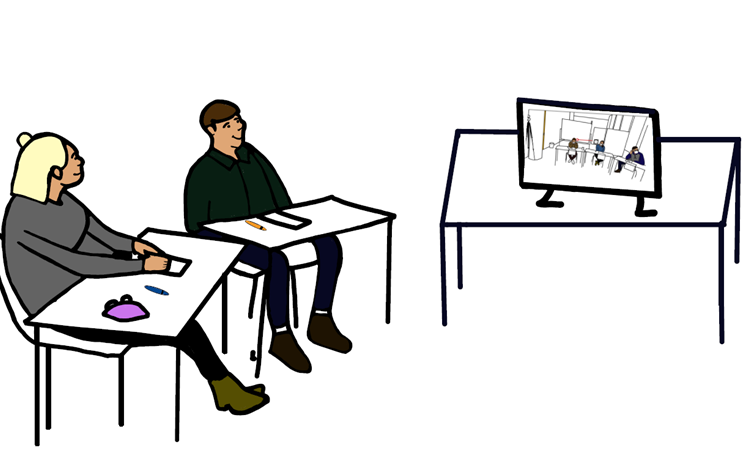
\includegraphics[width=0.45\textwidth]{appendix_figure2.png}
  \caption*{\textit{Note.} The experimenter and participant watched the previously taught micro-teaching unit on video.}
  \centering\caption{Laboratory setting of the interview.}
  \label{fig.a2}
\end{figure}

\begin{figure}[htbp]
  \centering
  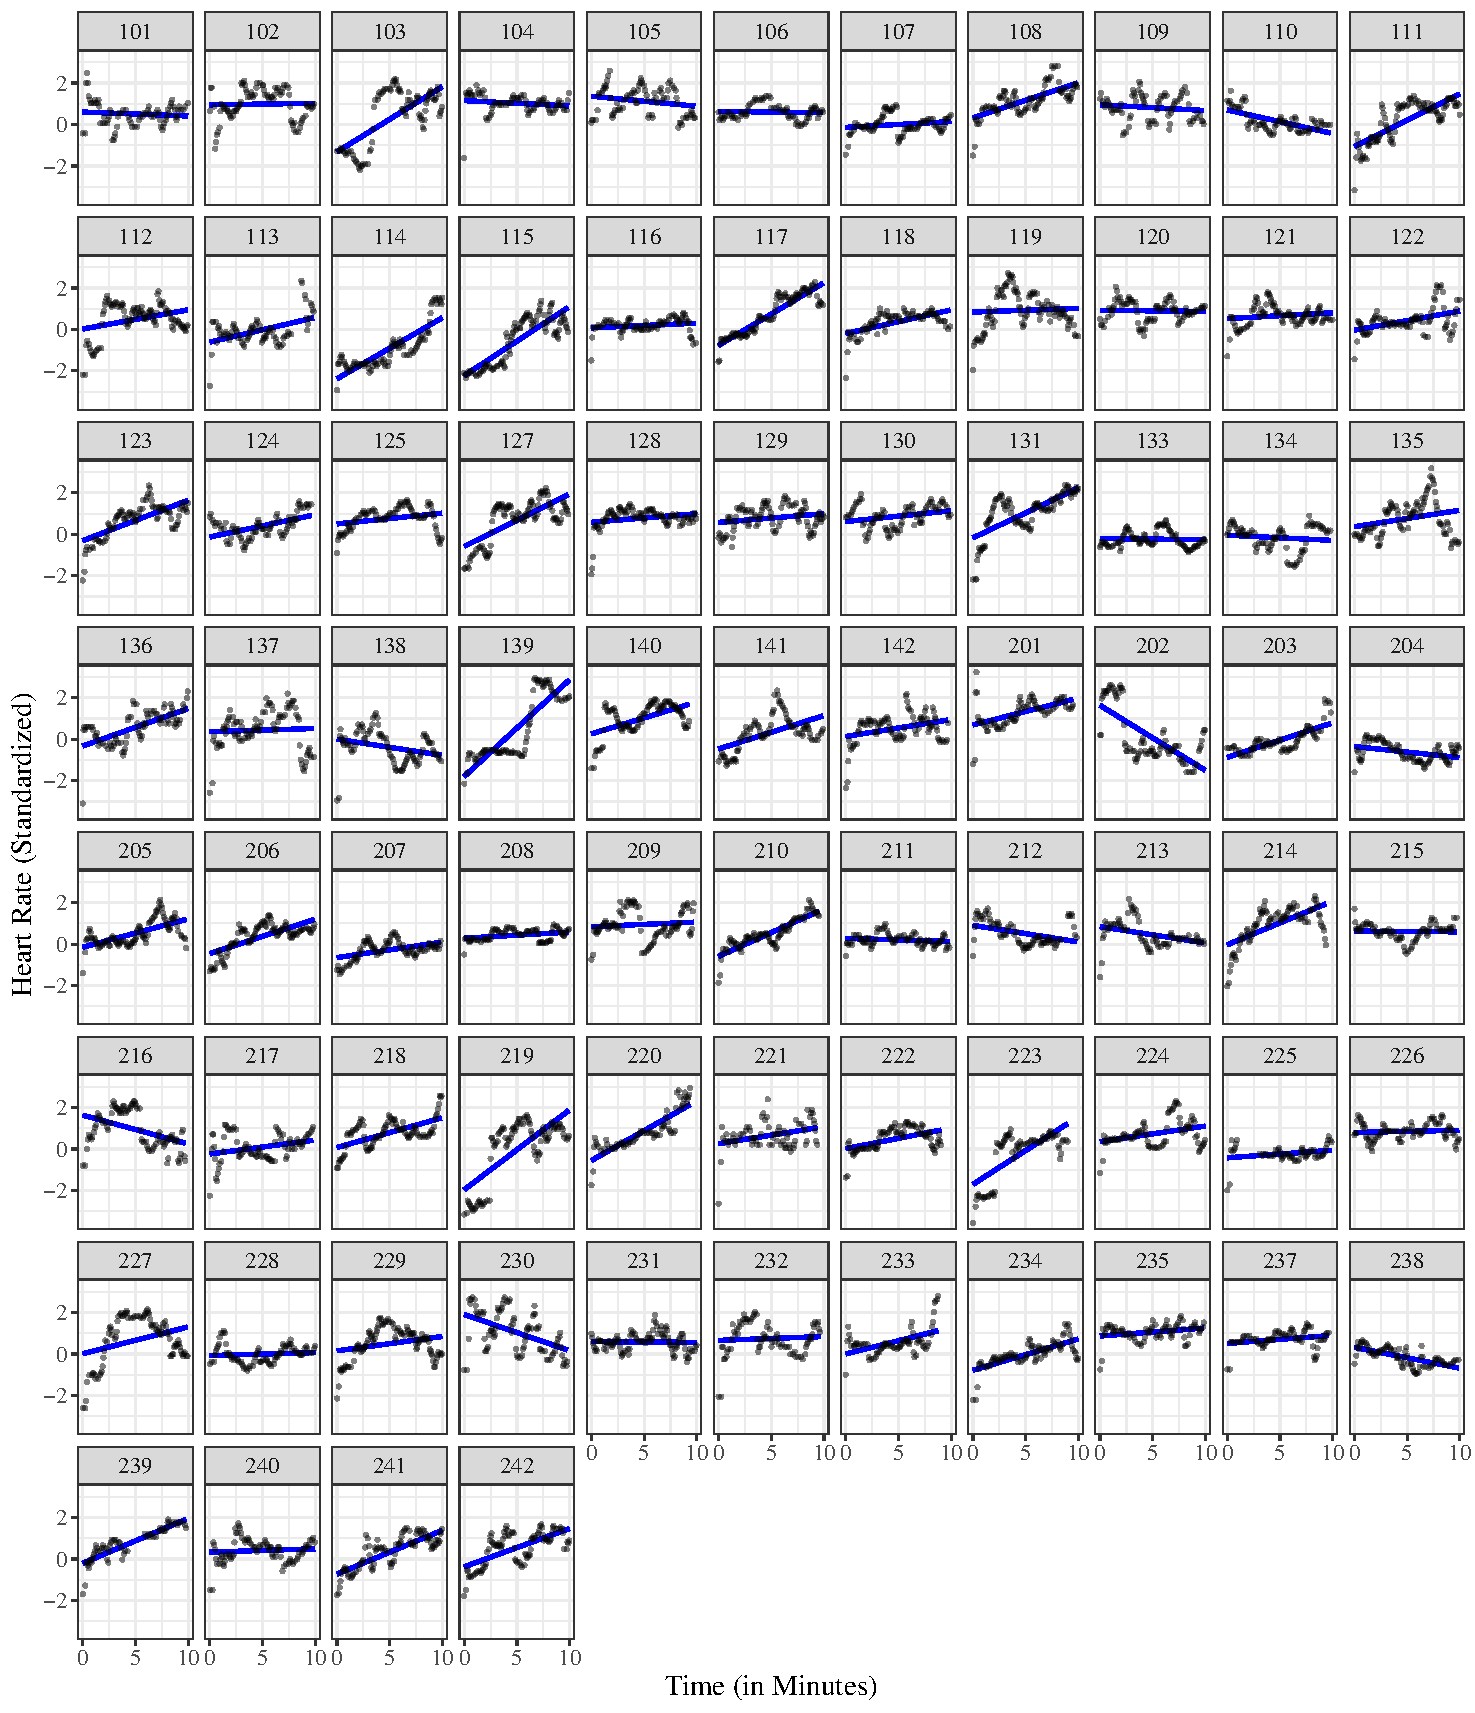
\includegraphics[width=1\textwidth]{plots_publication/plot_preparation_appendix.pdf}
  \caption{Linear estimation of individual HR changes over time during the preparation phase for $N$ = 81 participants. Each plot illustrates the mean standardized HR values (y-axis) across 10 minutes (x-axis), with the black dots representing observed HR data points and the blue line showing the estimated linear trend.}
  \label{fig.a3}
\end{figure}

\begin{figure}[htbp]
  \centering
  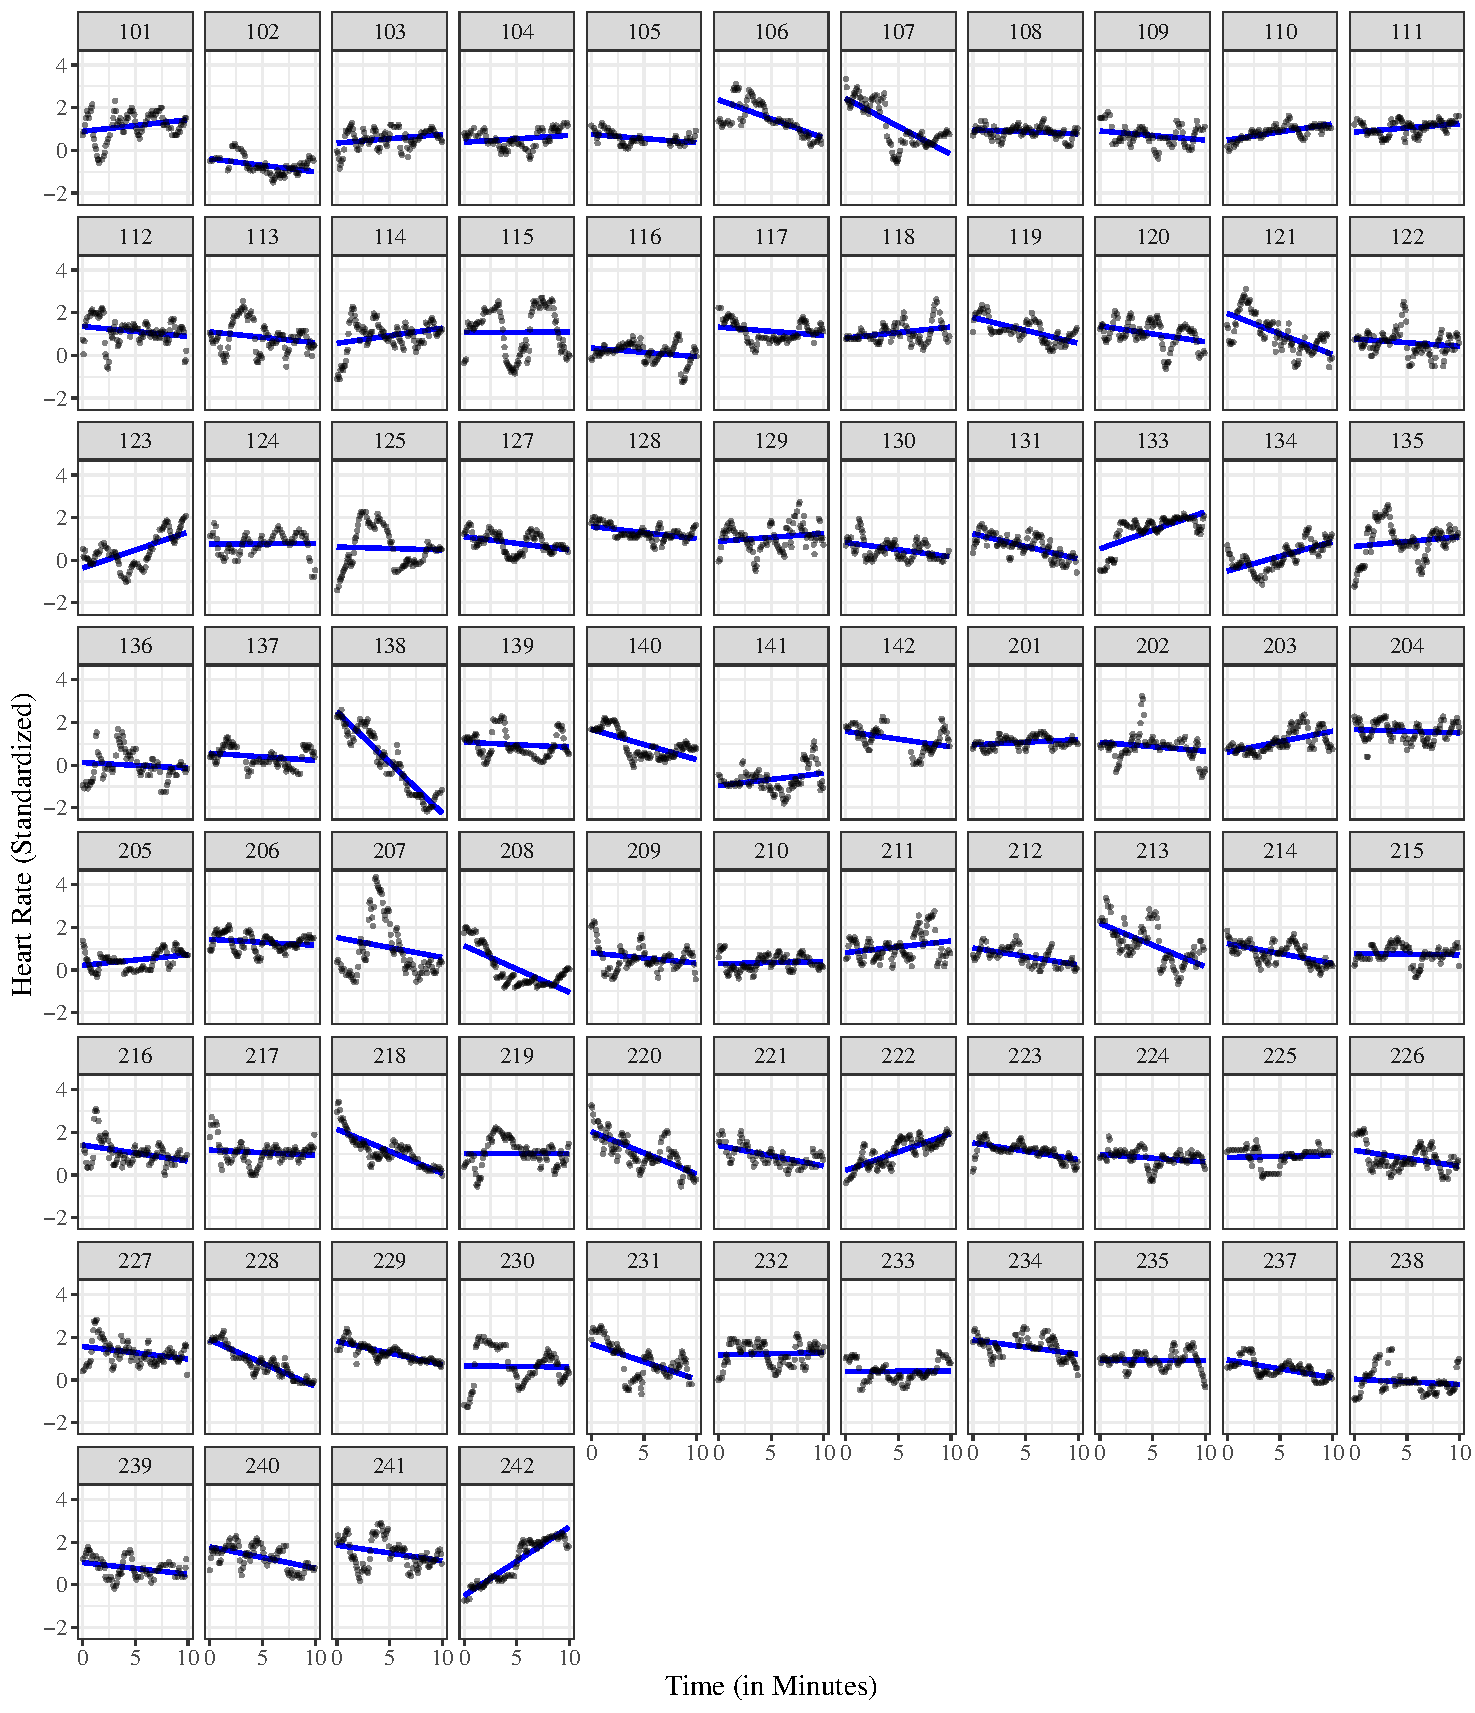
\includegraphics[width=1\textwidth]{plots_publication/plot_teaching_appendix.pdf}
  \caption{Linear estimation of individual HR changes over time during the teaching phase for $N$ = 81 participants. Each plot illustrates the mean standardized HR values (y-axis) across 10 minutes (x-axis), with the black dots representing observed HR data points and the blue line showing the estimated linear trend.}
  \label{fig.a4}
\end{figure}

\begin{figure}[htbp]
  \centering
  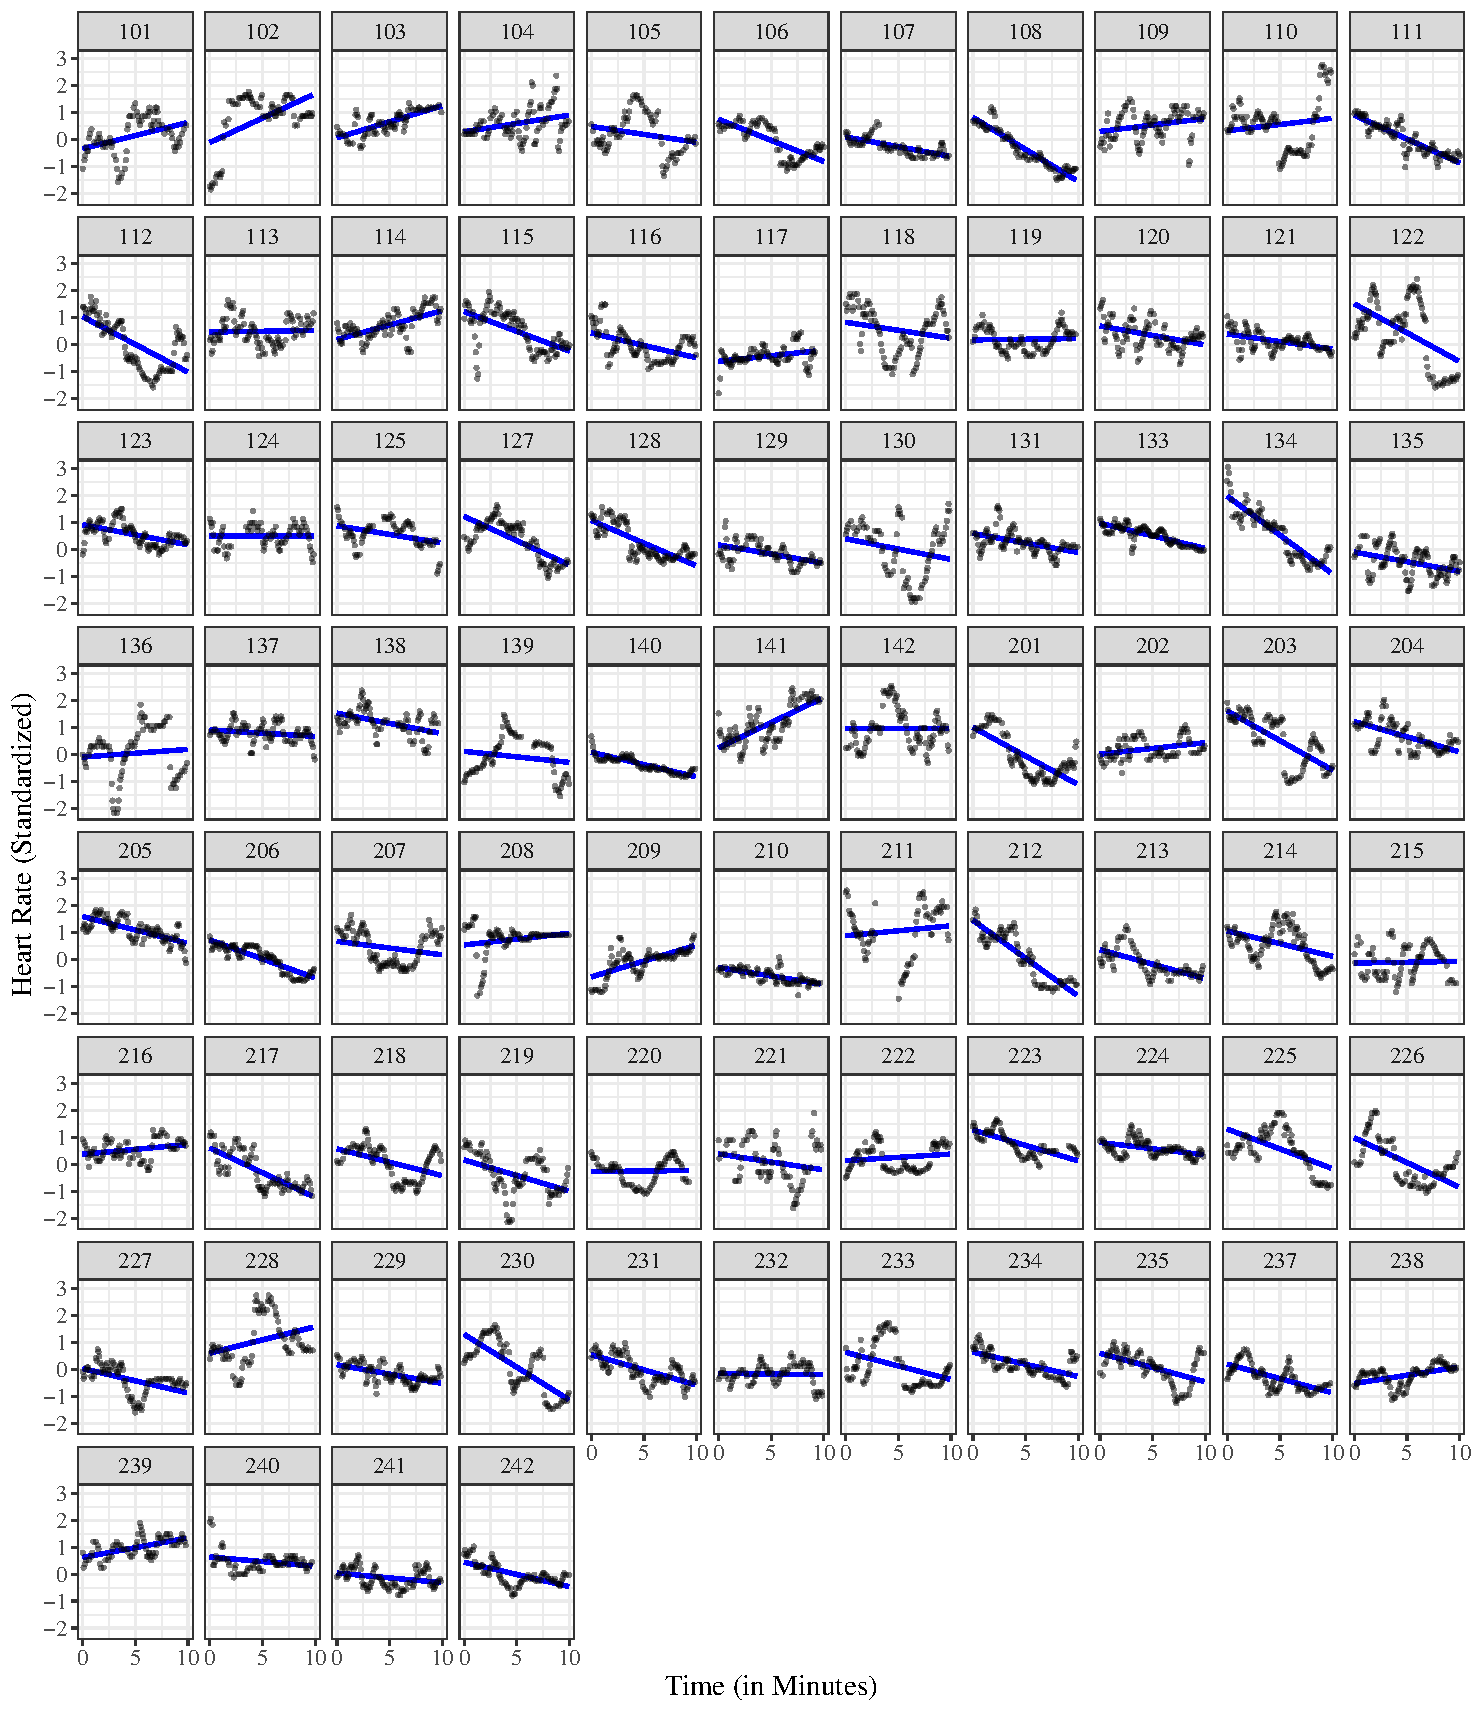
\includegraphics[width=1\textwidth]{plots_publication/plot_post_teaching_appendix.pdf}
    \caption{Linear estimation of individual HR changes over time during the post-teaching phase for $N$ = 81 participants. Each plot illustrates the mean standardized HR values (y-axis) across 10 minutes (x-axis), with the black dots representing observed HR data points and the blue line showing the estimated linear trend.}
  \label{fig.a5}
\end{figure}

\begin{figure}[htbp]
  \centering
  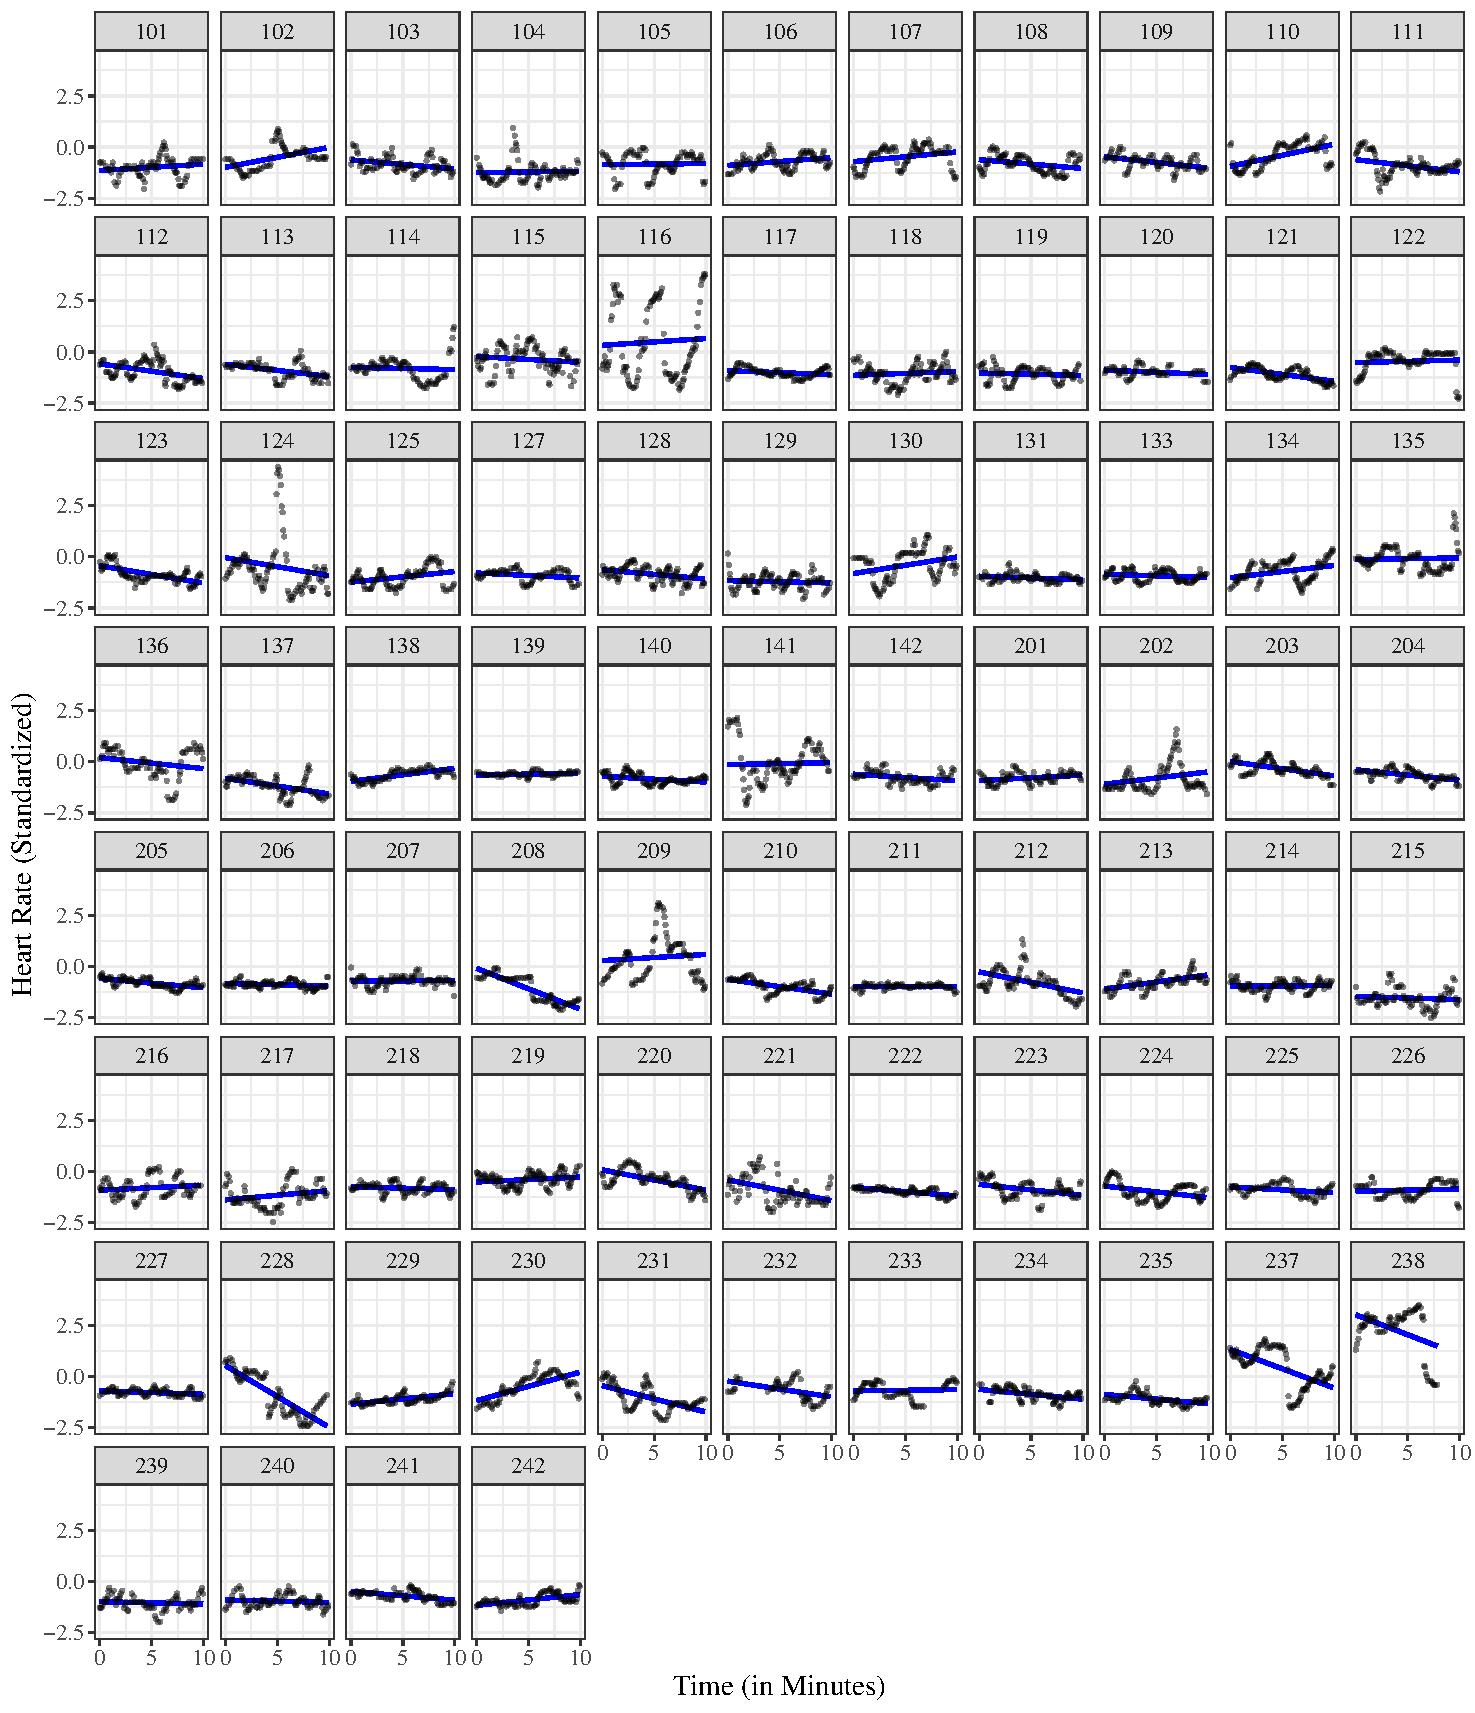
\includegraphics[width=1\textwidth]{plots_publication/plot_interview_appendix.pdf}
  \caption{Linear estimation of individual HR changes over time during the interview phase for $N$ = 81 participants. Each plot illustrates the mean standardized HR values (y-axis) across 10 minutes (x-axis), with the black dots representing observed HR data points and the blue line showing the estimated linear trend.}
  \label{fig.a6}
\end{figure}

\begin{figure}[htbp]
  \centering
  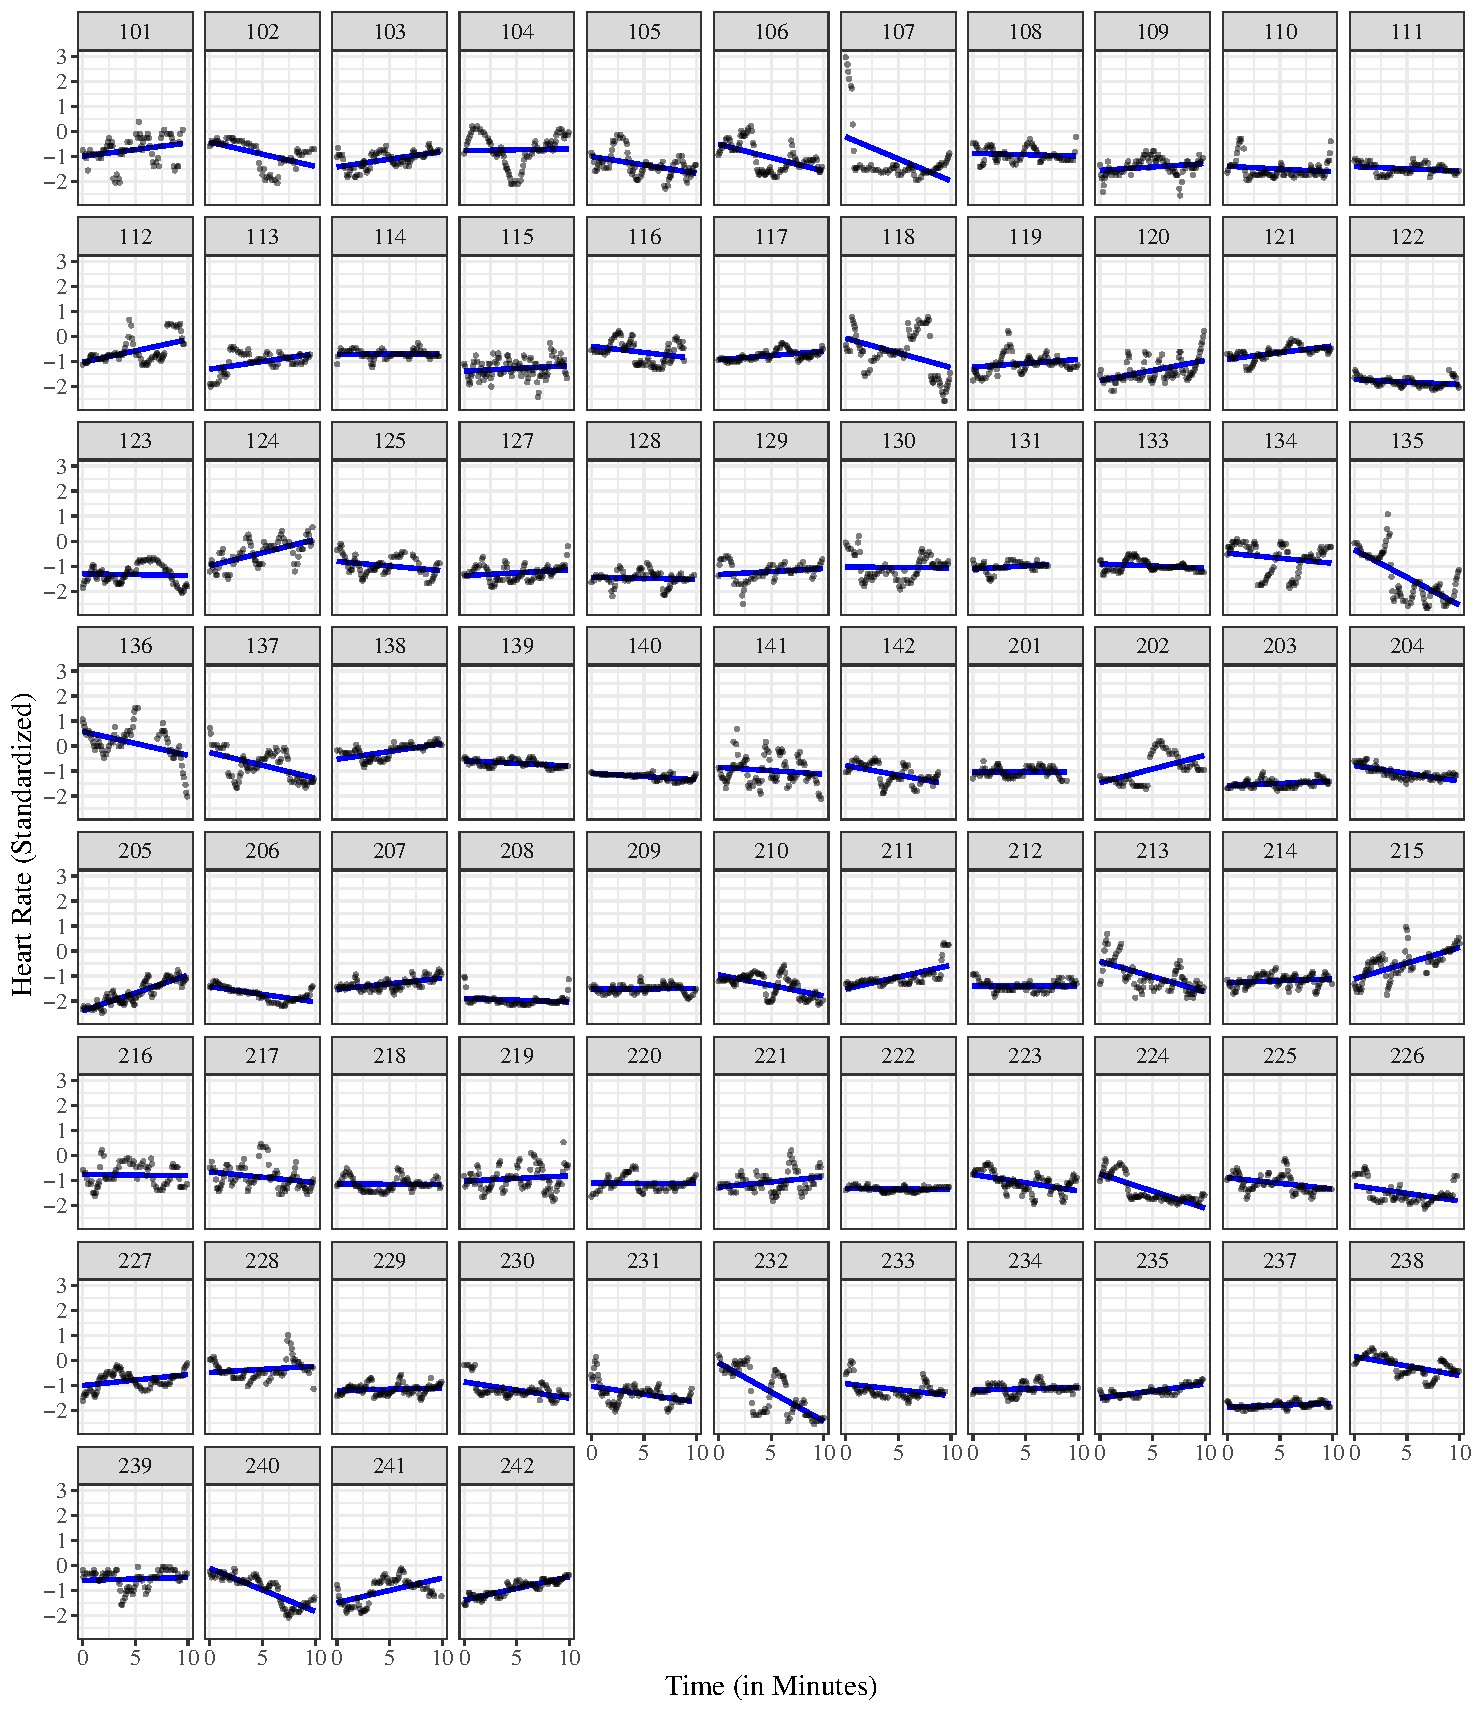
\includegraphics[width=1\textwidth]{plots_publication/plot_end_appendix.pdf}
    \caption{Linear estimation of individual HR changes over time during the end phase for $N$ = 81 participants. Each plot illustrates the mean standardized HR values (y-axis) across 10 minutes (x-axis), with the black dots representing observed HR data points and the blue line showing the estimated linear trend.}
  \label{fig.a7}
\end{figure}

\newpage

\bibliography{r-references.bib}


\end{document}
